\documentclass[preprint, review, 12pt]{article}

%%%%% kotex : 한글을 사용할 수 있는 환경을 제공함. 
\usepackage{kotex} 

%%%%% thm prop def proof solution등을 사용할 환경을 제공함. 
\usepackage{amsthm} %% amsthm : \newtheorem \theoremstyle 을 사용할 수 있는 환경을 제공함. 
%% 1) def, thm 등의 style을 제공. 
% plain 스타일
% def 스타일
\theoremstyle{definition}
\newtheorem{dfn}{Definition} 
%% section number에 따라서 count 한다는 의미. 만약 subsection number에 따라서 count하려면\newtheorem{dfn}{Def}[subsection]과 같이 하면 된다.   
\newtheorem{thm}{Thm}[section] 
\newtheorem{prop}[thm]{Proposition} %% thm과 counting number 공유 
\newtheorem{ex}{Example}[section]
\newtheorem{cmt}{Cmt}[section]
\newtheorem{rmk}{Remark}[section]
% remark스타일
\theoremstyle{remark}
\newtheorem{promise}{Promise}[section]

%% 2) proof, solution등의 style을 제공. 
\newenvironment{sol}{\begin{proof}[Solution]}{\end{proof}} %% solution을 proof처럼 사용할 수 있는 환경을 제공함.  


%%%%% 여러가지 수식관련 환경을 제공함. 
\usepackage{amsmath} % \align \alignat \multline 등의 명령을 사용할 수 있게 함. 
\usepackage{amsfonts} % \mathbb{R}를 사용할수 있게 함. 

%%%%% itemize관련 환경을 제공함. 
\usepackage{enumerate} %\begin{enumerate}[(i)]를 사용할수                                                                                                                                                                             있게 함. 

%%%%% 인용 
\usepackage{cite}

%%%%% 그림삽입
\usepackage{graphics} 
\usepackage{graphicx,lscape} %그림을 회전시켜삽입.
\graphicspath{{figure/}}%%%%% 그림들을 figure 에 정리할수 있게 함. graphicx 뒤에 선언해야함. 
\usepackage{subfig}
%\usepackage{subcaption} % 이것이 있어야지 subfigure를 사용할 수 있음. 
%%%%%% 모든문단에 들여쓰기를 하고 싶을 경우
\usepackage{indentfirst}

%%%%%% 글씨색 (color가 아니라 xcolor를 써야지 gray등의 색을 지정할 수있음) 
\usepackage{xcolor} 

%%%%%% 알고리즘 
\usepackage{algpseudocode}
\usepackage{algorithm}% http://ctan.org/pkg/algorithms

%%%%%% subsection을 많이 만들수 있는 패키지
\usepackage{titlesec}

%%%%%% 홈페이지, 참고도서등을 참조할 수 있는 패키지
\usepackage{cite, url}

%%%%%% \because \therefore를 사용할수 있게함. 
\usepackage{amssymb}

%%%%%% Operator정의 
\DeclareMathOperator*{\argmin}{arg\,min} %\usepackage{amsmath}를 써야지 정의가능함. 
\DeclareMathOperator*{\argmax}{arg\,max} %\usepackage{amsmath}를 써야지 정의가능함. 

%%%%%% 사용자정의 
\def\shrp{\paragraph{\textcolor{red}{\textit{\#.}}}}
\def\memo{\subparagraph{\textit{memo.}}}


\linespread{1.3}


\title{\bf Heavysnow Transformation} 
\medskip


\author{
\sc  Guebin Choi and Hee-Seok Oh\\ 
Department of Statistics\\
Seoul National University\\
Seoul 08826, Korea \\
\\
}
\date{Draft: version of \today}

\begin{document}

\maketitle

\newpage
\thispagestyle{empty}

\begin{center}
{\bf Abstract}
\end{center}
\noindent 
This paper presents a new multiscale transforms, termed 'heavy-snow transform', which is motivated by observing snow accumulation. Heavy-snow transform provides multiscale visualization which can capture the shape of land (or data structure) with different resolution. Some measures based on heavy-snow transform are newly defined to describe dissimilarity between data and the importance of data. Furthermore, some statistical applications are studied. 
\vskip 5mm
\noindent {\it Keywords}: Graph signal; Similarity; Distance; Multiscale method. 
\pagenumbering{arabic}
\newpage


\section{Introduction}
In this study we will propose a new method which can measure the distance between nodes in \emph{graph signal}. In here, graph signal $f$ is real valued function such that $f:{\cal V} \to \mathbb{R}$ where ${\cal V}$ is set of nodes (or vertices). We are interested in the distance or similarity(which is usually defined as the inverse of distance) in graph signal. 

Let $\nu_i$ and $\nu_j$ be a specific nodes in ${\cal V}$ and $f(\nu_1)$ and $f(\nu_2)$ be a value at $\nu_i$ and $\nu_j$. How to measure the similarity or disimilarity between $f(\nu_i)$ and $f(\nu_j)$? In other words, how can we define distance between $f(\nu_i)$ and $f(\nu_j)$?. The naive approach for measuring the distance between $f(\nu_i)$ and $f(\nu_j)$ is to use the Euclidean distance like: 
$
\|f(\nu_i)-f(\nu_j)\|_2:=\sqrt{(f(\nu_i)-f(\nu_j))^2}.
$ Of course, someone can use other measures such as Gaussian kernel weighting function. Those measures do not have a problem when they measure the distance of points which resides Euclidean space. However, it is reasonable to think that the graph signal resides in not only Euclidean space but also graph space. (Note that $f(\nu)\in \mathbb{R}$ but $\nu \in {\cal V}$.) The problem is here. Distance between $f(\nu_i)$ and $f(\nu_j)$ depends on disimilarity in Euclidean domains but distance between $\nu_i$ and $\nu_j$ depends on disimilarity in graph domains, which is determined by \emph{links} (or \emph{edges}), i.e., ${\cal E}$. However the methods presented above have limitations in that they do not consider the ${\cal E}$ when measuring the distance between observations. In here, considering \emph{links} between observation means that consider the structure of indices, i.e., ${\cal E}$. Let's move to Figure 1 to understand why you should consider the structure of index set in the graph signal. 

Figure 1 is made from example introduced in Shuman (2012). There are three graph signal in Figure 1. The interesting fact is that those three graph have exactly same $f(\nu_i)$ for each $\nu_i \in {\cal V}$. The only difference between them is ${\cal E}$ which are represented in dotted lines. Due to ${\cal E}$ all connected nodes in (a) seems to have a similar values but (c) is not. In other words, (a) looks like a low-frequency signal, while (c) looks like a high-frequency signal. (b) feels halfway between (a) and (c). You can easily check this is true by comparing the spectral density of (a)-(c) represented in second row of Figure 1. 

\begin{figure}[htbp]
\centering
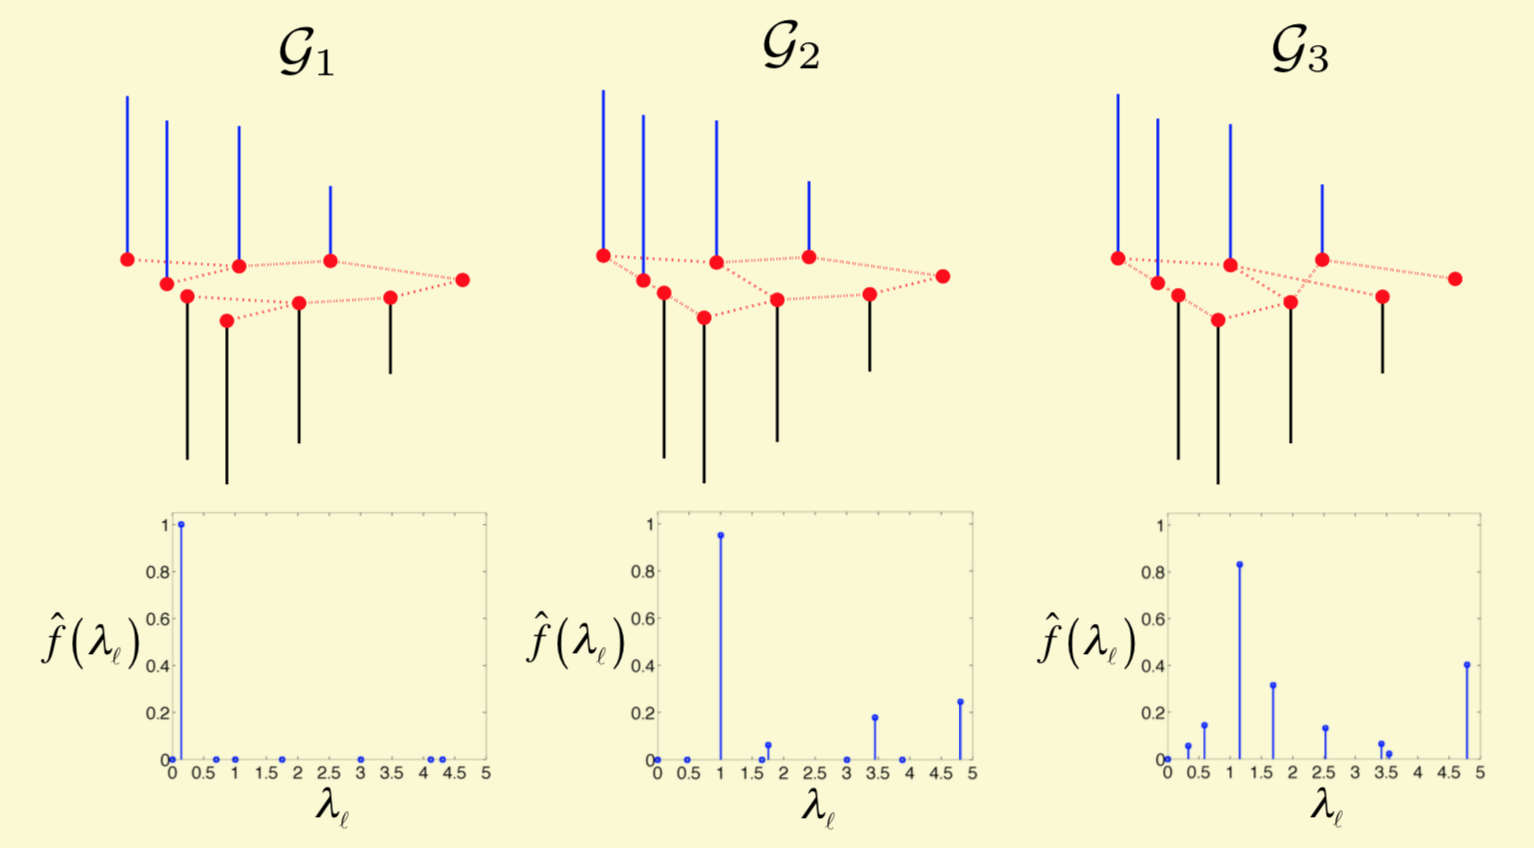
\includegraphics[width=1\textwidth]{Fig/Fig1.png} 
\caption{Example 1 in Shuman (2012)}
\end{figure}

The underlying structure of graph signal ${\cal E}$ affects distance between $\nu_i$ and $\nu_j$, and it affects the similarity (or disimilarity) between $f(\nu_i)$ and $f(\nu_j)$ as discussed in Figure 1. Therefore, when analyzing graph signal, measuring the distance between $\nu_i$ and $\nu_j$ is no less important than measuring the distance between $f(\nu_i)$ and $f(\nu_j)$. In other words, the distance in the graph domain is just as important as the distance in the Euclidean domain.

Various methods have been developed to measure the differences between nodes. The most common method is the shortest path, which measures the shortest distance between two nodes. Klein and Randić (1993) suggest the resistance distance which can measure the distance between nodes in undirected graph. Lafon and Lee (2006) suggest the diffusion distance. However, those methods have limitations such that they are only interested in distance between $\nu_i$ and $\nu_j$. That is, those methods could be suitable for graph $({\cal V},{\cal E})$ but not suitable for graph signal $f:{\cal V} \to \mathbb{R}$. 

Thus, our goal is that: Develope new distance considering the distance in vertex domain and the distance in the Euclidean domain simultaneously. To do this, we propose a new distance that takes into account the distance between the vertex domain and the distance from the Euclidean domain at the same time through an elegant technique called \emph{heavysnow transform}. We will formally define heavysnow transform in Section 2, instead, in this section, we will just breifly introduce the main idea and motivation of heavy transform. After that we will explain why our proposed distance is a reasonable measure which can properly mix the information of the graph and Euclidean domains. 

The heavysnow transform is invented by observing snow accumulation over the land or ground. In this study, you can consider the ground as graph signal $f$ and snow as some positive constant $b$ we will stack on $f$. Let $\tau$ be the number of falling snow. Our propose distance, named \emph{snow distance}, is defined 
\[
sdist(\nu_i,\nu_j; \tau):=\mathbb{E}\| h(\nu_i; \tau )- h(\nu_j;\tau)\|_2.
\]
In here, $h(\nu_i;\tau)$ will be defined more strictly at Section 2. In this section, you can consider $h(\nu_i;\tau)$ as the updated value of $f(\nu_i)$ after $\tau$. In other words you consider $h(\nu_i;\tau)$ as snowy ground. If we set $\tau=2$, then $h(\nu_i;\tau)$ will be one of $f(\nu_i)$, $f(\nu_i)+b$ and $f(\nu_i)+2b$. 

As you can see, when $\tau = 0$, the snowdist between two nodes $\nu_i$ and $\nu_j$ becomes $\|f(\nu_i)-f(\nu_j)\|_2$, which is exactly same as Euclidean distance. However, as $\tau$ increases, the snow distance starts to mix the distance in the Euclidean domain and the distance in the graph domain. That is, as $\tau$ increases, the structure of ${\cal E}$ is additionally reflected in dissimilarity between $f(\nu_i)$ and $f(\nu_j)$. This is the key to considering both graph and Euclidean domains simultaneously. 

How is this possible? This is due to the very unique feature of snow accumulation. For your easy and intuitive understanding, let's see Figure 2. In Figure 2-(a), (b), and (c), the curved lines which are located in the bottom of each figure represents ground or graph signal $f$. If you put a less viscous material like rain on $f$, it would look like (a). If we add a highly viscous material to $f$, it would look like (c). If material has medium viscosity like snow, it would look like (b). In other words, to have a shape like (b), the snow stacked on $v_i$ with following characteristics: 
\begin{enumerate}[(i)]
\item Snow can flow to adjacent areas.
\item Snow cannot flow to higher ground. 
\end{enumerate}
Note that (i) needs the information of ${\cal E}$, i.e., it needs information of graph domain since (i) is determinded by whether or not $v_i$ and $v_j$ are connected.  On the other hand, (ii) relates to the values of $f(v_i)$ and $f (v_j)$ which is information of Euclidean domain. Therefore, the process of snow accumulation can be reproduced only with the information of both domains. As a result, the distance between snowy ground $h(\nu_i,\tau)$ and $h(\nu_j,\tau)$ is surprisingly mixed with information from both domains. (This is covered more closely in Section 2.)

If the viscosity is too high, the shape of the snow accumulations will always like (c), regardless of the structure of the index set ${\cal E}$. This is the result of considering only the values defined in the Euclidean domain and ignoring the graph domain information. Conversely, (a) tends to ignore information in the Euclidean domain too much. In (b), the information from the Euclidean domain and the vertex domain are well balanced.

\begin{figure}
\centering
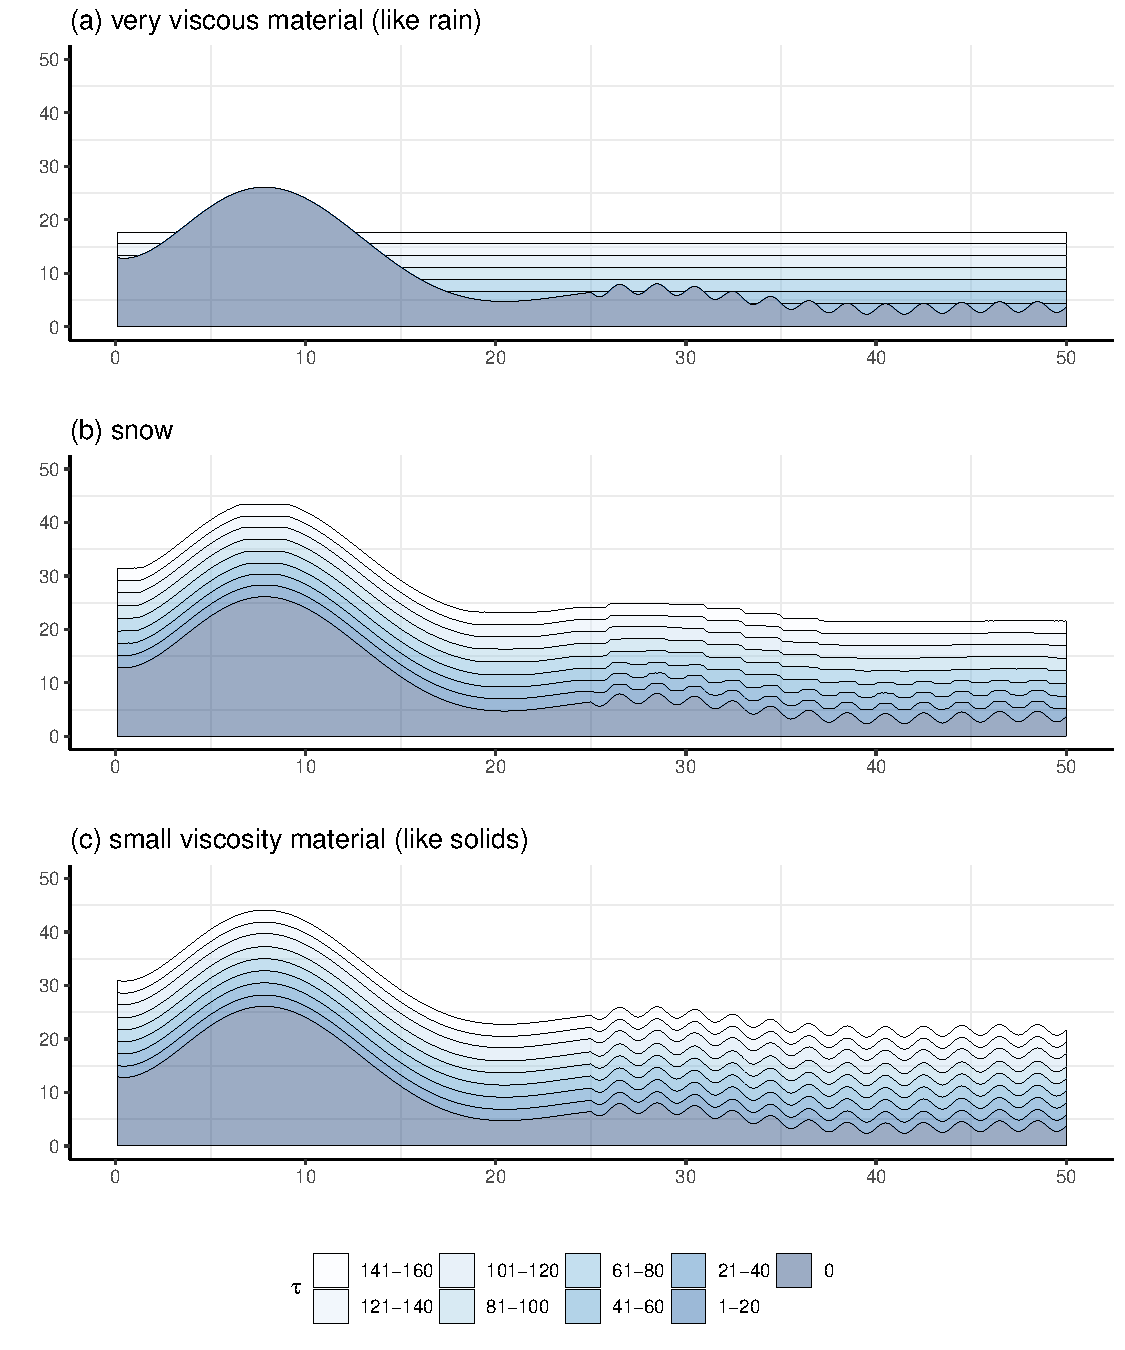
\includegraphics[width=1\textwidth]{Fig/Fig2.pdf}
\caption{The underlying signal and accumulations with different viscosity. In here, $\tau$ represent that amount of stacked accumulations.}
\end{figure}

The remaining of this paper is organized as follows. Section 2 defines heavy-snow transformation and proposes some statistics based on heavysnow transformation. 
Section 3 introduces some visualization techniques that can effectively show the results of heavysnow transform. Section 4 presents possible applications of heavysnow with various numerical experiments and real data analysis. Finally, concluding remarks are given in Section 5 where a possible use for smoothing is briefly discussed as a future research topic. 

\section{Heavy-Snow Transformation}
\subsection{Definition of Heavy-Snow Transformation}
Before defining heavy-snow transformation, we would like to explain data structure to which the transformation is applicable. 
Let ${\cal V}$ be set of nodes (or vertices) and ${\cal E}$ be set of links (or edges). In the context of heavy-snow transformation, the link means a way that snow can move in. Basically, you can consider ${\cal V}=\{\nu_1,\dots,\nu_n\}$ as given index set such as ${\cal V}=\{1,2,\dots,n\}$. However, it is often reasonable to view node as realization of some random variable $X$. This can be illustrated by setting node as $v=X(\nu)$. 

Let $X:{\cal V} \to {\cal M}$ be a random variable where ${\cal M}$ is isometrically embedded manifold in $\mathbb{R}^{N}$. Supposed that we observed $v_1,v_2,\dots,v_n ~\sim~ i.i.d. ~ F_X$ where $F_X$ is cumulative distribution functions of $X$. The graph signal $f$ is real valued function such that 
\[
f : {\cal M} \to \mathbb{R}.
\]
Furthermore, we define a set of linked vertices with a particular vertex $v_i$ as ${\cal N}_{v_i}=\{v_j: (\nu_i,\nu_j) \in {\cal E} \}$ where $\nu_i:X^{-1}(v_i)$.
Note that $\forall M \in {\cal M} : ~ V^{-1}(M) \in \sigma(X)$ where $\sigma(X)$ is smallest $\sigma$-field which makes $X$ as random variable. Thus $X^{-1}(v_i)$ is always well defined. 

%Basically, the information of the set of linked vertices determines the data structure. For example, in one-dimensional data or time series, we can define the set of linked values as ${\cal N}_{v_i}=\{v_{i-1},v_{i+1}\}$.  

From now on, we explain how to implement the phenomenon of snow accumulation. Let's come back to Figure 2 for easy understanding. Figure 2 (a), (b) and (c) show different viscous materials stacked on the same ground. For the case of Figure 2 (a), material flows to local minimum, which might be similar to the accumulation of rainwater. On the other hand, the material in Figure 2 (c) does not flow and just stacks up above ground. The most important property of the material in (a) is `continue to flow until blocked'. Note that small viscous materials do not accumulate. Those small viscous materials such as water accumulate only when they reach the local minimum. On the other hand, the most important property of highly viscous materials such as (c) is `stacking.' They only accumulate and never flow. 

The snow can be interpreted as having a medium viscosity between two materials of Figure 2 (a) and (c), as metioned in Section 1. In order to express the viscosity of the snow, we assume that snow has both feature of (a) and (c). In other words, snow continues to accumulate AND flow until blocked. 
For your easy understanding let's assume some specific situation as follows: 

\begin{enumerate}[1.]
\item (snow falls) Draw $v_i$ from $V$ with probability $\frac{1}{n}$. Suppose that snow falls at $v_i$ as much as $b$. 
\item (accumulation) Like (c) snow stacks on $v_i$. Thus, in this case, value of $v_i$, i.e., $f(v_i)$ will be updated by $f(v_i)+b$. 
\item (flows/blocked) After that snow can move to one of ${\cal N}_{v_i}$ which is neighborhood of $v_i$. Of course, if ${\cal N}_{v_i}=\emptyset$, the snow will no longer flow. However, ${\cal N}_{v_i}\neq \emptyset$ does not necessarily mean that snow can flow (since snow cannot flow high). Thus, we should compare value of $f(v_i)+b$ and $f(v_j)$ to check flowbility of snow. In otherwords, we should check ${\cal U}_{v_i}:={\cal N}_{v_i} \cap \{v_j: f(v_j) \leq f(v_i)+b\}$ is emptyset or not. 
\begin{itemize}
\item (flow) In the case of ${\cal U}_{v_i}\neq\emptyset$, which is an unblocked situation, snow (which stays in $v_i$) can flow to $v_j$ that is randomly sampled element from ${\cal U}_{v_i}$ with probability $\frac{w_{ij}}{\sum_{j \in {\cal U}_{v_i} }w_{ij} }$. 
\item (blocked) If ${\cal U}_{v_i}=\emptyset$, which is a blocked situation, snow can't flow anymore. In this cases, the next node is randomly selected from $V=\{v_1,\dots,v_n\}$ with probability $\frac{1}{n}$. 
\end{itemize}
\item In the cases of `flows', go back to step 1 and repeat above procedure with assuming that snow falls at $v_j$ (which is element of ${\cal U}_{v_i}$) as much as $\gamma b$. In here $\gamma \in (0,1)$ is parameter adjusting viscosity of snow. (If you choose very small $\gamma$, shape of snow accumulation will be (c) in Figure 2.) For `blocked' situation, go back to step 1 with assuming that snow falls at $v_j$ (which is randomly selected node in $V$) as much as $b$.
  
\end{enumerate}

The following is the formal definition of heavy-snow transform.
\begin{dfn}\label{snow:df_hst}
Let $V:=\{v_i:i=1,2,\dots,n\}$ be the given index set or realization of $X$. For fixed $i$, let ${\cal N}_{v_i}$ be set of linked values with $v_i$ and $f(v_i)$ be function valued mapped to $v_i$ and $\boldsymbol f$ be ${\boldsymbol f}=\{f(v_i): i=1,\dots,n \}$. Let $b$ be the amount of falling snow and $\tau$ be the number of falling snows. Let $\{v^{(0)},v^{(1)},\dots,v^{(\tau)}\}$ as \emph{trace of snow} where $v^{(0)}$ is result of randomly select from $V$ with probability $\frac{1}{n}$ and $v^{(\tau)}$ is defined
\[
v^{(\tau)}=\begin{cases}
\mbox{ sample from } {\cal U}_{v^{(\tau-1)}} \mbox{ with probability } \frac{w(v^{(\tau-1)},v^{(\tau)})}{\sum_{j \in {\cal N}_{v^{(\tau-1)}}}w(v^{(\tau-1)},v^{(\tau)})}  & {\cal U}_{v_{(\tau-1)}}\neq \emptyset \\ 
\mbox{ sample from } V \mbox{ with probability  } \frac{1}{n}  & {\cal U}_{v_{(\tau-1)}}= \emptyset 
\end{cases}
\]
For any $\tau \in \{1,\dots,n\}$, the $\tau$-th \emph{snowyground} of ${\boldsymbol f}$ is defined by 
\[
{\boldsymbol h}^{(\tau)} := {\boldsymbol h}^{(\tau-1)}+{\boldsymbol \xi}^{(\tau)}
\]
where ${\boldsymbol h}^{(0)}={\boldsymbol f}$ and ${\boldsymbol \xi}^{(\tau)}=\{\xi^{(\tau)}(v_i): i=1,\dots,n\}$ is amount of stacked snow at $\tau$ whose elements are defined by 
\[
\xi^{(\tau)}(v_i)=	\begin{cases}
\gamma \xi^{(\tau)}(v_{(\tau-1)})  & {\cal U}_{v_{(\tau-1)}}\neq \emptyset \\ 
b &  {\cal U}_{v_{(\tau-1)}} = \emptyset. \\ 
\end{cases}
\]
Define operator ${\cal H}$ called \emph{heavy-snow transform} such that
\[
{\cal H}{\boldsymbol f}:=\begin{bmatrix} 
h^{(0)}(v_1) & h^{(1)}(v_1) & \dots & h^{(\tau)}(v_1) \\ 
h^{(0)}(v_2) & h^{(1)}(v_2) & \dots & h^{(\tau)}(v_1) \\ 
\dots  & \dots & \dots & \dots \\ 
h^{(0)}(v_n) & h^{(1)}(v_n) & \dots & h^{(\tau)}(v_n) \end{bmatrix}
\]
and call the matrix ${\cal H}{\boldsymbol f}$ as \emph{heavy-snow} of ${\boldsymbol f}$. 


\subsection{Snowdistance and some properties} 
\begin{dfn}
Let ${\boldsymbol f}$ be the graph signal on weighted graph $(V,E,W)$. Let ${\cal H}{\boldsymbol f}$ be heavysnow for ${\boldsymbol f}$ with some $\tau$, $\gamma$ and $b$. The \emph{snow distance} between $v_i$ and $v_j$ is defined by 
\[
sdist(v_i , v_j) := E\|{\boldsymbol h}_i- {\boldsymbol h}_j\|_2.
\]
where ${\boldsymbol h}_i=\big(h^{(0)}(v_i),\dots,h^{(\tau)}(v_i)\big)$ is $i$-th row of ${\cal H}{\boldsymbol f}$.
\end{dfn}

Suppose following model:
\[
f(v_i)=g(v_i)+\epsilon_i, ~ i=1,2,\dots,n. 
\]
Let ${\cal H}\boldsymbol{f}$ be a heavysnow transform of ${\boldsymbol f}$. Since $f(v_i)$ is random variable ${\boldsymbol h}_i$ can be thought as random vector (\textcolor{red}{need to prove}) such that 
\[
{\boldsymbol h}_1,\dots,{\boldsymbol h}_n \sim F_{\boldsymbol h}.
\] 
\shrp HST에서 ${\boldsymbol h}$는 우리가 데이터로 부터 얻어낼 수 있는 모든 정보를 포함하고 있다고 볼 수 있다. 따라서 스무딩이나 클러스터링등은 모두 ${\boldsymbol h}$에서 얻어지는 통계량 $T(F;\tau)$로 정의가능하다. 여기에서 $T(F;\tau)$ 아래와 같은 functional $T:{\cal A} \to \mathbb{R}$ 이다. 
\[
T(F;\tau):=\int g({\boldsymbol h}) dF({\boldsymbol h})
\]
, where $F({\boldsymbol h})=\mu_1(-\infty,h_1]\times \dots \times \mu_{\tau+1}(-\infty,h_{\tau+1}]$ , $\mu:=P \circ {\boldsymbol h}^{-1}$ 이고 ${\cal A}$ 는 $(\Omega,{\cal F})$ 에서 정의가능한 모든 finited-signed measure 들의 집합 혹은 그것의 convex subset 이다. 

- 이때 $T$ 에 대한 ***($\tau+1$)-dimensional influence function*** 은 아래와 같이 정의한다. 
\begin{align}
IF({\boldsymbol h}; T,F,\tau)= \lim_{t\downarrow 0}\frac{T\Big((1-t)F(\boldsymbol{h}) + t \delta(\boldsymbol{h}) \Big)-T(F(\boldsymbol{h}))}{t}
\end{align}
우리는 아래와 같이 $IF({\boldsymbol h}; T,F,\tau)$의 ***sample version*** 을 생각해 볼 수 있다. 
\begin{align}
SC_{n}({\boldsymbol h};\tau)= \frac{T\Big((1-1/n)F_{n-1}(\boldsymbol{h}) + 1/n ~ \delta(\boldsymbol{h}) \Big)-T(F_{n-1}(\boldsymbol{h}))}{1/n}
\end{align}
보는것처럼 $SC_{n}$은 $IF({\boldsymbol h}; T,F,\tau)$ 의 정의에서 $t$ 대신에 $1/n$을, $F$ 대신에 $F_{n-1}$을 대입하여 얻을 수 있다. 보통 $SC_{n}$ 를 ***sensitivity curve*** 라고 부른다. 

- ***claim 1.*** **(1)** 각각의 노드 $v_i$에서 정의된 확률변수 $f(v_i)$가 서로 독립이고 같은분포를 가진다고 하자. 그리고 **(2)** 각 노드에 연결된 edge의 수가 동일하다고 하자(이런 그래프를 ***regular graph*** 라고 함). 그러면 $\boldsymbol{h}(v_i)$ 역시 서로 독립이고 같은 분포를 가질것이다. $F_n$을 $\boldsymbol{h}(v_1),\dots,\boldsymbol{\dot h}(v_n)$에 대응하는 empirical-cdf 라고 하자. 글리벤코-칸텔리정리는 $F_n \to F$ 임을 보여준다. 따라서 적당히 큰 $n$에 대하여 $F_n$은 $F$의 neighborhood에 속한다고 볼 수 있다. 따라서 
\begin{align}
T(F_n) & \approx  T(F)+\int IF(\boldsymbol{h},T,F)d(F_n-F)(\boldsymbol{h}) \\
& = T(F)+\int IF(\boldsymbol{h},T,F) dF_n(\boldsymbol{h}) 
\end{align}
이다. 여기에서 $\int IF(\boldsymbol{h},T,F)dF(\boldsymbol{h})=0$ 임이 사용되었다. 따라서 
\begin{align}
\sqrt{n}\Big(T(F_n)-T(F) \Big) \to N(0,V(T,F))
\end{align}
이다. 여기에서 $V(T,F)=\int IF(\boldsymbol{h},T,F)^2 dF(\boldsymbol{h})$ 이다. 

- ***claim 2.*** claim 1에서 $V(T,F)$ 는 $\tau \to \infty$ 일 경우 $0$ 으로 수렴한다. 왜냐하면 $\tau$ 가 커질수록 
\begin{align}
\boldsymbol{h}(v_1)\approx \boldsymbol{h}(v_2) \approx \dots \approx \boldsymbol{h}(v_n)
\end{align}
와 같이 되기 때문이다. 

- claim 1에서 **(2)** 의 조건은 생략불가능하다. 즉 $f(v_i)$가 서로 독립이고 같은 분포를 가진다는 것이 반드시 $\boldsymbol{h}(v_i)$ 들이 서로 독립이고 같은분포를 따른다는 것을 임플라이 하지는 않는다. 

- 노드간의 snow-dist 역시 $\boldsymbol{h}(v_i)$ 의 함수이므로 $T$로 표현가능하다. 따라서 (1),(2) 를 가정하면 노드간의 snow-dist 역시 $N(0,V(T,F))$ 를 따른다. 즉 (1),(2) 아래에서 노드간의 snow-distance 를 히스토그램으로 그려보면 정규분포와 비슷한 모양이 된다. 이때 snow-dist들의 평균거리가 0으로 수렴한다는 조건이 추가적으로 있으면 claim2 에 의해서 모든 노드들이 한점으로 뭉쳐버리게 된다. 

- 거리들의 히스토그램이 정규분포처럼 보이지 않는 경우는 (1) 이 성립하지 않거나 (2) 가 성립하지 않기 때문이다. 그렇다면 각각의 거리가 정규분포처럼 보이는 그룹이 2개가 있다면 이것은 (1) 혹은 (2) 가 성립하는 그룹이 2개 있다고 해석해도 될까? 아래가 성립하면 이렇게 주장할 수 있을것이다. 

- ***claim 3.*** 모든 $\tau$에 대하여 아래를 만족하는 거리 (혹은 유사거리) $d^* $ 가 존재한다. 
\begin{align}
d_1 \big(\boldsymbol{h}(v_i),\boldsymbol{h}(v_j)\big) = d^* \big(F^* (f(v_i)),F^* (f(v_j))\big)
\end{align}
여기에서 $F^* (x) :=\mu_1(-\infty,x]\times \mu_1(-\infty,\infty] \dots \times \mu_{\tau+1}(-\infty,\infty]$ 이고 $\mu:=P \circ {\boldsymbol h}^{-1}$ 이다. 

\subsection{discussions}

\shrp ${\cal M}$을 compact smooth manifold 라고 가정하자.  그리고 ${\cal M}$은 어떤 $\mathbb{R}^{N}$공간에 isometrically embedded 되어 있다고 가정한다. 즉 ${\cal M} \subset \mathbb{R}^N$ 이다.  만약에 3차원 공간에 표현된 구의 표면을 표현하고 싶다면 아래과 같이 설정할 수 있다. 
\[
\mathbb{R}^3 : \mbox{3차원공간} 
\]
\[
{\cal M} : \mbox{구의 표면을 나타내는 매니폴드}
\]
그리고 ${\cal M}$ 과 같이 유클리드 공간에  isometrically embedded 된 매니폴드를 리만매니폴드라고 한다(아마도).  

\shrp 라플라스 연산자는 아래와 같이 정의한다. 
\[
\triangle f =\triangledown^2 f
\]
라플라스 벨트라미 오퍼레이터를 아래와 같이 정의하자. 
\[
\Delta {\cal M}
\]

\shrp 그래프 $(V,W)$는 어떠한 매니폴드의 $({\cal M},{\cal W})$ 의 sample version이라고 하자.  아래의 성질을 만족하는(이것이 맞는 표기법인지 모르겠다. 이런식으로 가정하는 논문을 찾아봐야 할것 같음) 상황에서만 이론을 전개할 것이다. 
\begin{align}
{\cal G} \to {\cal M} \quad as~ n\to \infty 
\end{align}
신호처리식 언어로 표현하면 샘플링 주기가 $0$에 가까워지면 distrcret signal 이 continuous signal 로 수렴한다는 의미이다. 이때 샘플링은 일정한 간격으로 할 수도 있지만 어떤 특정확률에 따라서 랜덤하게 샘플링할 수도 있다. 따라서 기븐 그래프 ${\cal G}=(V,E)$ 가 어떠한 매니폴드의 sample version 이라고 볼 수 도 있지만 어떠한 랜덤엘리먼트의 ***realization*** 이라고 볼 수 도 있다. 

우리의 정의에서 $b$는 밴드윗의 역할을 한다. ***asymptotic property*** 를 증명하기 위해서는 밴드윗이 0으로 간다는 조건이 필수적인데 HST의 아이디어로 비춰볼때 이 조건은 
\begin{align}
\|{\cal N}_ i\|\to \infty \quad \mbox{ for all } v_i \in V
\end{align}
와 비슷하다. 

벨킨의 논문에서 ${\cal M}$ 은 유클리드 스페이스 $\mathbb{R}^{N}$에 ***isometric*** 하게 임베딩된 ***compact and smooth*** 매니폴드라고 가정한다(벨킨, 2008, p.1290). 이러한 가정은 매니폴드에서 샘플된 자료들에 대한 엣지를 고려하지 않고 단순히 거리만으로 유사성을 따지기 위함이다. 심지어 유클리디안거리를 그대로 쓰기 위하여 아이소메트릭 가정을 하였다. (컴팩트 and 스무스 가정은 왜 했는지 잘 모르겠음 아마 벨트라미-라플라시안을 잘 정의하기 위함일것으로 추측됨) 아무튼 이러한 셋팅하에서 ${\cal G} \to {\cal M}$ 를 모순없이 가정할수 있는것 같다. 우리는 위의 가정들을 쓰지 않는 대신에 ${\cal M}$ 위에서 적당하게 샘플을 잘하면 그래프가 매니폴드를 근사한다고 직접 가정한다. 구체적으로는 아래와 같은 가정이 될것 같다. 
\begin{align}
\frac{\|{\cal N}_ i \|}{n} \overset{\operatorname{pr} }{\to} \int_{v \in {\cal N}(v_i)}dP_{\cal M}(v)
\end{align} 
여기에서 $P_{\cal M}$ 는 매니폴드 ${\cal M}$ 위에서 정의된 메져이다. 

- ***claim*** 여기서는 given ${\cal M}$ 에 대하여 특정한 확률로 ${\cal G}$ 가 뽑힌 경우를 고려한다. $f:{\cal M} \to \mathbb{R}$ 이라고 하자. $P_{\cal M}$ 를 ${\cal M}$ 에서 정의된 ***probability measure*** 라고 하고 $p_{\cal M}$ 을 $P_{\cal M}$ 에 대응하는 ***probability density function*** 이라고 하자. 이제 $v_1,\dots,v_n$을 $P_{\cal M}$에 따라 ${\cal M}$ 에서 추출된 어떠한 sample 이라고 하자. $f(v_i)$를  랜덤이 아니라고 하자. 
\begin{align}
{\bf Lf}(v_i):=\frac{1}{\|{\cal N}_ i\|}\sum_{j \in {\cal N}_ i} e^{ -\frac{d_1^2(v_i,v_j)}{2b^2} } \big(f(v_i)-f(v_j)\big)
\end{align}
이때 $v_i \in {\cal M}$ 주변의 점들을 ${\cal N}(v_i)$ 라고 하자(이것은 ${\cal N}_ i$의 continuous 버전이라고 볼 수 있음). 만약에 $\int_{v \in {\cal N}(v_i)} dP(v)>0$ 이면 $n \to \infty$ 일때 $\|{\cal N}_ i \| \to \infty$ 가 성립할것 같다.
그리고 이러한 조건 하에서 아래가 성립할것 같다. 
\begin{align}
{\bf Lf}(v_i) \overset{\operatorname{pr}}{\rightarrow}\frac{1}{\mbox{something} }\int_{ {\cal N}(v_i)} e^{ -\frac{d_1^2(v_i,v)}{2b^2} } \big(f(v_i)-f(v)\big)dP_{\cal M}(v)
\end{align}
여기에서 someting은 bandwidth $b$와 관련있는 어떠한 상수일것같다. 만약에 ${\cal M}$이 유클리드공간에 임베딩된 매니폴드라면 우변이 ${\cal L}_ {\cal M}f(v_i)$ 와 관련이 있을 것이다. 여기에서 ${\cal L}_ {\cal M}$은 라플라스-벨트라미 연산자이다. 일단은 아래가 성립한다고 생각하자. 
\begin{align}
{\bf Lf}(v_i) \overset{\operatorname{pr}}{\rightarrow} {\cal L}_ {\cal M}f(v_i)
\end{align}

\iffalse
\subsection{Statistical Measure of Heavy-Snow Transform}

A bottom curve in Figure \ref{snow:motivatingex} represents $X_i$ and other curves represent the snowy ground, $Y_{i,\tau}$ with various $\tau$. The interesting thing is that if $X_i$ and $X_j$ have a different local structure, then $\{Y_{i,\tau}\}_{\tau=0}^{\cal T}$ and $\{Y_{j,\tau}\}_{\tau=0}^{\cal T}$ also have a different sequence. Therefore, we can express a dissimilarity of $X_i$ and $X_j$ as distance between $\{Y_{i,\tau}\}_{\tau=0}^{\cal T}$ and $\{Y_{j,\tau}\}_{\tau=0}^{\cal T}$.

\begin{dfn}
	Let $\{X_i\}$ be the given data and ${\cal N}_{i}$ be a set of linked values with $X_i$. Let  $\{Y_{i,\tau}\}_{\tau=0}^{\cal T}$ be the heavy-snow transform on $(\{X_i\},\{{\cal N}_i\})$. A dissimilarity between $X_i$ and $X_j$ is defined as
	\[
	d_{\cal T}(X_i,X_j)=E\left[\rho\left(\{Y_{i,\tau}\}_{\tau=0}^{\cal T},\{Y_{j,\tau}\}_{\tau=0}^{\cal T}\right)\right], 
	\]
	where $\rho\left(\{Y_{i,\tau}\}_{\tau=0}^{\cal T},\{Y_{j,\tau}\}_{\tau=0}^{\cal T}\right)=\|(Y_{i,0},\dots,Y_{i,{\cal T}})-(Y_{j,0},\dots,Y_{j,{\cal T}}) \|_2^2.$
\end{dfn}

Based on the definition of dissimilarity, we define an importance of each observation.

\begin{dfn}
	Let $\{X_i\}$ be the given data and ${\cal N}_{i}$ be a set of linked values with $X_i$. Let $d_{\cal T}(X_i,X_j)$ be the dissimilarity between $X_i$ and $X_j$. For fixed $\delta>0$, an importance of specific observation $X_{k}$ is defined as 
	\[
	imp(X_{k},{\cal T})=\frac{\left|\{X_{j}:d_{\cal T}(X_{k},X_{j})>\delta\}\right|}{\left|\{X_i\}\right|}, 
	\]
	where $|A|$ is the cardinality of set $A$. 
\end{dfn}

Note that if $X_i=c(\in \mathbb{R})$ for all $i$, then $d_{\cal T}(X_i,X_j)=0$ for all $i,j$, which implies that all data points have the same importance. If $\delta \to \infty$, then $imp(X_i,{\cal T}) \to 0$ for all $i$; thus, the entire data points are not important. If $\delta \to 0$, then $imp(X_i,{\cal T}) \to 1$ for all $i$, so it means that all of data points are important. Hence, it is necessary to choose an  appropriate $\delta$ to measure the importance of the data. 
\fi 
\section{Visulization}

\section{Numerical Experiments}
\subsection{Simulated Examples}
In this section, we present some examples of heavy-snow transforms with one-dimensional data. For all examples, we set  ${\cal N}_i=\{X_{i-1},X_i,X_{i+1}\}$, $b=0.02\times \sqrt{V(\{X_i\})}$ and $p_{ij}=\frac{1}{3}$. 
\vskip 3mm
\noindent\textbf{Example 4.1}:
Consider following Gaussian process $\{X_i\}$ generated by $N(\mu_i,0.5)$, where 
\[
\footnotesize{\mu_i=\left\{
	\begin{array}{ll}
	0, &~1\le i \le 200\\
	1, &~201\le i \le 300\\
	0,&~301\le i \le 700\\
	5, &~701\le i \le 800\\
	0, &~801\le i \le 1000.\\
	\end{array}
	\right.}
\]
\begin{figure}
	\centering
	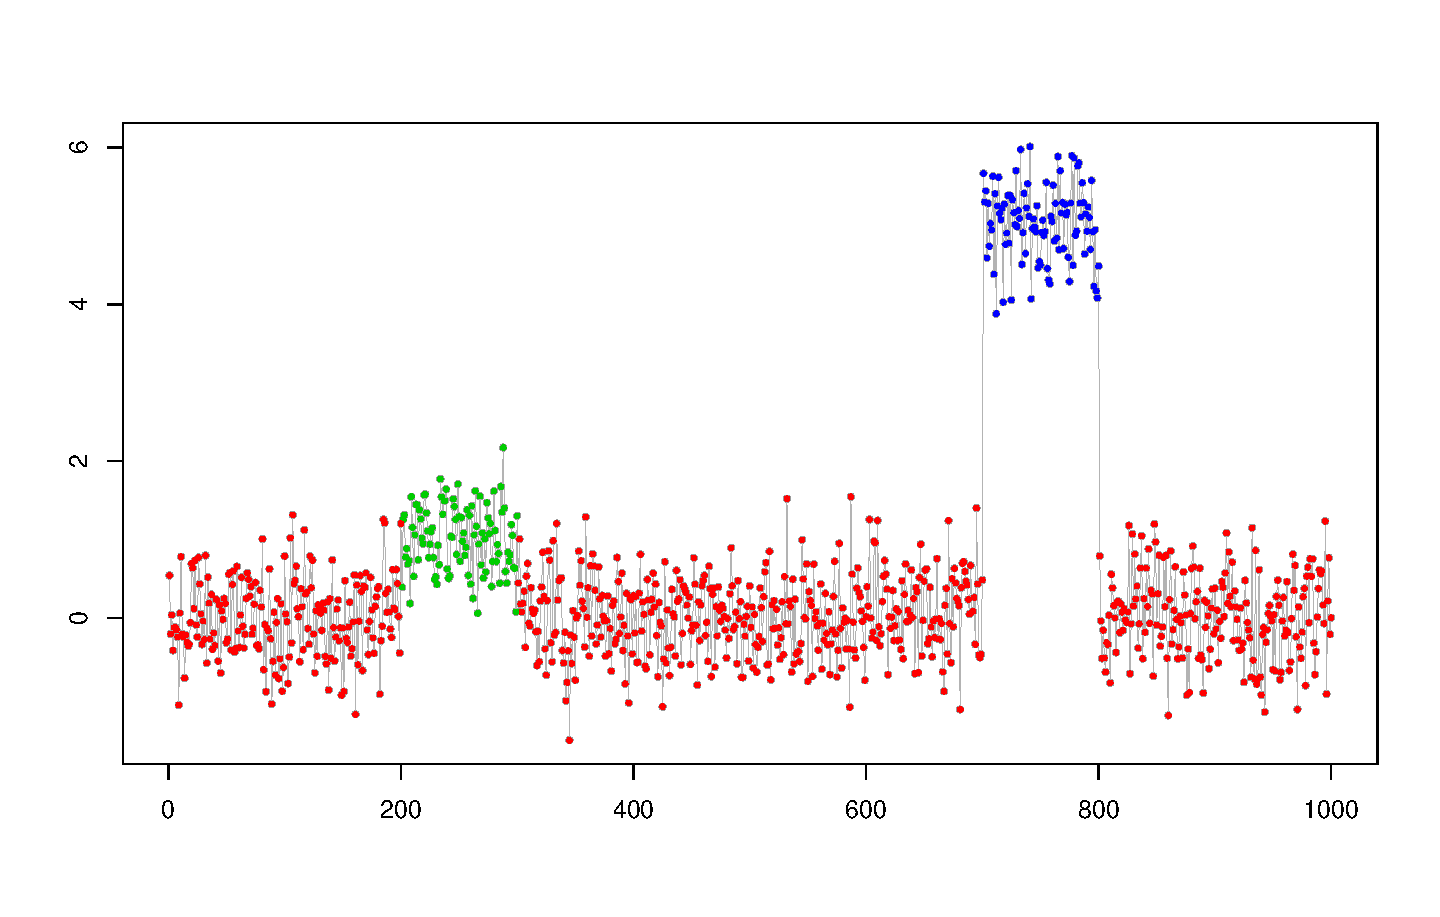
\includegraphics[width=1\textwidth]{Fig/snow_ex1_fig1.pdf}
	\caption{$X_i$ in Example 4.1.} 
	\label{snow:ex1_1}
\end{figure}
Figure \ref{snow:ex1_1} shows a realization of $X_i$, where observations with $\mu=1$ are marked as green and observations with $\mu=5$ are marked as blue.

\iffalse
\begin{sidewaysfigure}
	\centering
	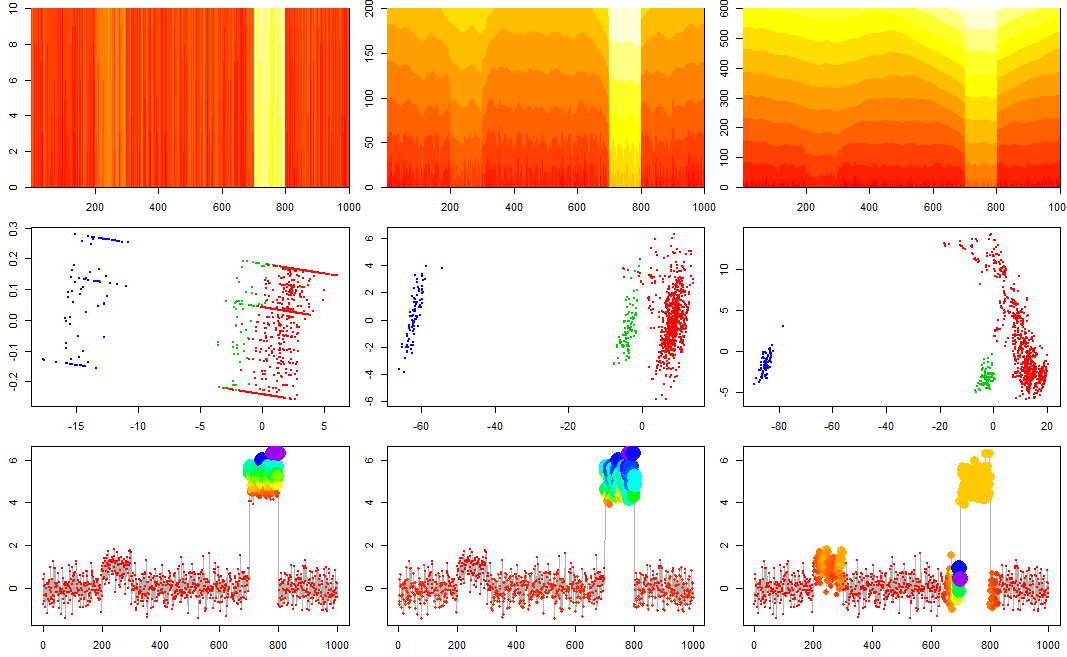
\includegraphics[width=0.75\textwidth]{Fig/snow_ex1_fig2.png}
	\caption{\textbf{Top:} Plot of heavy-snow transform: $(i,\tau,Y_{i,\tau})$ with ${\cal T}=10$ (left), ${\cal T}=200$ (middle), and ${\cal T}=600$ (right). 
		\newline
		\textbf{Middle:} Principal component plot of $\{Y_{i,\tau}\}_{\tau=0}^{\cal T}$ with ${\cal T}=10$ (left), ${\cal T}=200$ (middle), and ${\cal T}=600$ (right).
		\newline
		\textbf{Bottom:} Plot of $(i,X_{i})$ with $imp(X_i,{\cal T})$. In here $imp(X_i,{\cal T})$ are represented in color and size with ${\cal T}=10$ (left), ${\cal T}=200$ (middle),  and ${\cal T}=600$ (right).}
	\label{snow:ex1_2}
\end{sidewaysfigure}
\fi

The first row in Figure \ref{snow:ex1_2} is the result of the heavy-snow transform with ${\cal T}=10,~200$ and $600$, where the x-axis represents the index of the data, the y-axis represents $\tau$, and the color represents the value of $Y_{i,\tau}$. As one can see, $\{Y_{i,\tau}\}_{i=1}^{1000}$ with small $\tau$ represents $\{X_i\}$ with high-resolution and $\{Y_{i,\tau}\}_{i=1}^{1000}$ with large $\tau$ represents $\{X_i\}$ with low-resolution. Thus, this map is clearly a multiscale representation. 

The second row in Figure \ref{snow:ex1_2} shows principal component plot of $\{Y_{i,\tau}\}_{\tau=0}^{\cal T}$ with different $\cal T$. Note that blue and red/green ones are well separated in x-axis. Thus, it can be interpreted that the first principal component is thought of as an overall average of data. The interpretation of the second principal component could be more difficult than first one. It is related to the structure of linked data, that is, the land-shape. To understand the meaning of second principal component, suppose that snow falls as much as $\tau=1$. Then value of $E(Y_{i,1}-X_i)$ is perfectly determined by considering structure between $X_{i-1},X_{i}$ and $X_{i+1}$. So, the values of $E(Y_{i,1}-X_i)$ are divided by the following types of land-shapes:
\begin{enumerate}[(i)]
	\item local minimum: $X_i=\min(X_{i-1},X_i,X_{i+1})$
	\item local maximum: $X_i=\max(X_{i-1},X_i,X_{i+1})$
	\item flat: $X_{i-1}=X_i=X_{i+1}$ 
	\item uphill: $X_{i-1}<X_i<X_{i+1}$
	\item downhill: $X_{i-1}>X_i>X_{i+1}$
	\item flat-uphill: $X_{i-1}=X_i<X_{i+1}$ or $X_{i-1}>X_i=X_{i+1}$
	\item flat-downhill: $X_{i-1}=X_i>X_{i+1}$ or $X_{i-1}<X_i=X_{i+1}$
\end{enumerate}
Note that for all $i$, $P(X_{i-1}=X_i)=0$ in this example. Thus, we could not consider (iii), (vi) and (vii). Note also that values of $E(Y_{i,1}-X_i)$ are the same in the cases (iv) and (v). Thus, the values of $E(Y_{i,1}-X_i)$, amount of snow accumulation, can be roughly divided into three groups according to the land-shapes and these are represented in three straight lines in the left panel of the second row. 

The second row in Figure \ref{snow:ex1_2} also contains a multiscale concept. In ${\cal T}=10$, data can be roughly divided into two groups, blue one and red/green ones. And each group can also be divided into three groups according to land-shape. If one increases the scale up to ${\cal T}=200$, in other words, if you more widely consider the linked data, then groups of blue, green, and red dots are clearly distinguished, compared to ${\cal T}=10$. Instead, three straight lines disappear, so we no longer know whether each observation is local maximum or minimum. In other words, we lose some local-scale information. Now, let's move the principal component plot with ${\cal T}=600$, which shows the most global-scale analysis. We easily check that there are some points at which the value of the second principal component is very high. These points are located in the neighborhood of $i=700$ or $i=800$, which are the points where sudden mean changes occur. Note that detecting these points need more wide consideration about linked data. So these points are not separated from the main group in the local-scale analysis. 

For a fixed $\delta$, an importance of specific point $X_{k}$ can be calculated by counting how many points are in $\{X_j:,d_{\cal T}(X_{k},X_{j})>\delta\}$. In this example, we choose $\delta$ as the median of $\{d_{\cal T}(X_{i},X_{j}): i,j \in \{1,\dots,1000\} \}$. Results for calculation importance of data are shown in the third row. Importance is marked by various colors and sizes. Bigger ones are more important than small ones and purple ones are more important than red ones. The interesting thing is that importance of data changes over scales. In the local-scale analysis, observations which are located in $i \in (700,800)$ are considered to be important. However, in the global-scale analysis, observations where sudden mean change occurs (such as $i=700$ or $i=800$) are considered to be more important. 
\vskip 3mm
\noindent\textbf{Example 4.2}:
Consider a Gaussian process $\{X_i\}$ generated by $N(\mu_i,0.5)$, where 
$${\mu_i=\left\{
	\begin{array}{ll}
	0, &~1\le i \le 512\\
	5, &~513\le i \le 1024.\\
	\end{array}
	\right.}$$
Figure \ref{snow:ex2_1}(a) shows a realization of $X_i$, where red, green, blue, light blue and purple colors represent $\{X_i\}_{i=1}^{472}$,  $\{X_i\}_{i=473}^{502}$, $\{X_i\}_{i=503}^{522}$, $\{X_i\}_{i=523}^{552}$ and $\{X_i\}_{i=553}^{1024}$, respectively. As one  can see, the data have a single change point in $i=513$ and blue ones contain this sudden mean changes. Green and light blue ones are the neighborhood of the change point. Figure \ref{snow:ex2_1}(b) shows principle component plot of $\{Y_{i,\tau}\}_{\tau=0}^{\cal T}$, where ${\cal T}=120$. The red ones and purple ones are separated from each other. Thus, data with $\mu_i=0$ and $\mu_i=5$ are well separated in ${\cal T}=120$. We would like to emphasize that the green, blue and light blue ones are also separated from their main groups because they are located around the change point. So which points are important in Figure \ref{snow:ex2_1}(b)? One can easily check that red and purple area are denser than the areas where green, light blue and purple are located. So the importance of $\{X_i\}$ will be high in the neighborhood of the change point. Figure \ref{snow:ex2_1}(c) shows $(i,imp(X_i,120)) $, the importance plot. Here, we choose $\delta$ as the median of $\{d_{{\cal T}=120}(X_{i},X_{j}): i,j \in \{1,\dots,1000\} \}$ as in Example 4.1. As expected, $imp(X_i,120)$ has a peak in $i=512$, where the sudden mean change occurs. Figure \ref{snow:ex2_1}(d) shows another importance plot as in the third row of Figure \ref{snow:ex2_1}. 
\begin{figure}
	\centering
	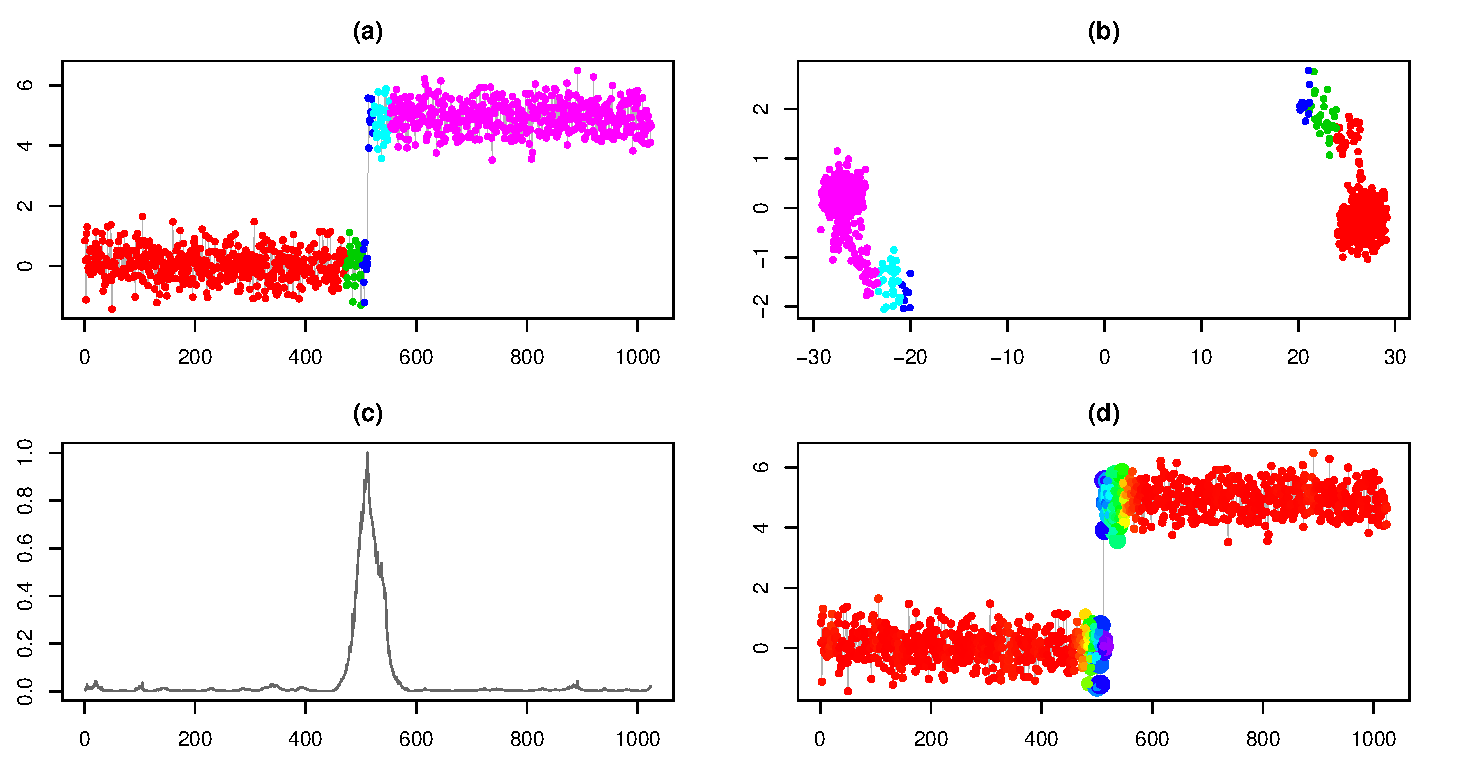
\includegraphics[width=1\textwidth]{Fig/snow_ex2_fig1.pdf}
	\caption{(a) $X_i$; (b) Principal component plot of $\{Y_{i,\tau}\}_{\tau=0}^{120}$; (c) Plot of $(i,imp(X_i,120))$; (d) Plot of $(i,X_i)$ where $imp(X_i,120)$ are marked color and size.}
	\label{snow:ex2_1}
\end{figure}

Furthermore, the importance of $X_i$ can be applicable to a smoothing problem that estimate $\mu_i$ from $X_i$. The following is the proposed smoothing procedure. 
\begin{itemize}
	\item[1. ] Calculate the importance of $X_i$, i.e., get the $imp(X_i,{\cal T})$. 
	\item[2. ] For $b=1,\dots,B$, get $X_i^{(b)}$ such that 
	\[
	X_i^{(b)}=\begin{cases} X_i, & i \in M \\ 
	\tilde{X}_i, & i \in M^c,
	\end{cases}
	\]
	where $M$ is length-$N_0(<N)$ samples without replacement from a population of $\{1,2,\dots,N\}$ with weight $$\mathbf{w}=\left(imp(X_i,{\cal T}),\dots,imp(X_N,{\cal T})\right)$$ and $\tilde{X}_i$ is linearly interpolated value from $\{X_i\}_{i\in M}$. 
	\item[3. ] Get $\hat{\mu}_i=\frac{1}{B}\sum_{b=1}^{B}X_i^{(b)}$ 
\end{itemize}
The key of the above procedure is that we do not use random sampling. Instead, we consider the importance of data as sampling weight. Thus, the important data is more likely to be sampled than other. 

Figure \ref{snow:ex2_2} shows the smoothing results. Left-top panel shows the original data. The red line in the left-bottom denotes a  wavelet fit by EbayesThresh (Johnstone and Silverman 2005). The green line in right-bottom represents a wavelet fit by SURE threshold (Donoho and Johnstone 1994). The result by our proposed method is shown as the yellow line in the right-top panel. In this example, we choose $\cal T$ as $120$ and $N_0=50$. As one can see, the performance of the proposed method is comparable to  the wavelet fits and we want to emphasize that our method is not limited to the data structure. 

\begin{figure}
	\centering
	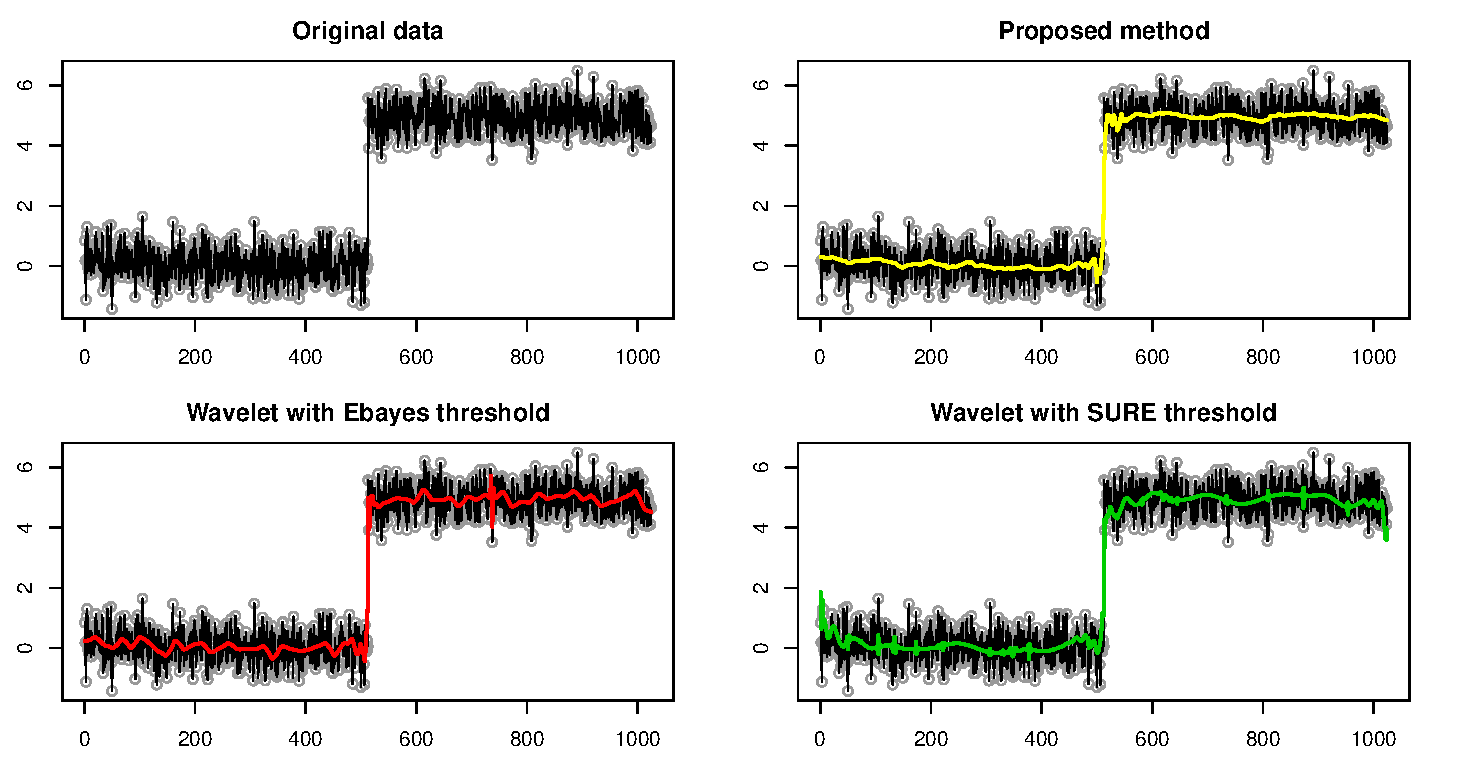
\includegraphics[width=1\textwidth]{Fig/snow_ex2_fig2.pdf}
	\caption{Smoothing results} 
	\label{snow:ex2_2}
\end{figure}


\subsection{Real Data Analysis}
\subsubsection{Avenger's}
\noindent\textbf{\underline{Data dercription}}

\noindent\textbf{\underline{What movie is important?}}

Leskovec (2009) : 연구그룹들을 네트워크화해서 중심연구그룹(?)을 찾았음. 

\noindent\textbf{\underline{Decomposition}}

\subsubsection{Les Misérables}
\noindent\textbf{\underline{Data dercription}}

\noindent\textbf{\underline{Who is important in Les Misérables?}}

\subsubsection{Earthquake}
\noindent\textbf{\underline{Data dercription}}

\noindent\textbf{\underline{Smoothing}}

\subsubsection{Distribution of Species of Animals} 
\noindent\textbf{\underline{Data dercription}}

\noindent\textbf{\underline{Smoothing}}

\noindent\textbf{\underline{Where do the habitats overlap?}}

\subsubsection{Seoul Metro data}
\noindent\textbf{\underline{Data dercription}}

In this example, we analyze subway passenger data of Seoul Metro Line 2 on March 7, 2014, which is represented in Figure \ref{snow:subway_in_0}. In this figure, $x$-axis denotes station, $y$-axis represents time, and color shows the number of people to get on Line 2. As one can see, each cell looks highly associated with vertical ones and horizontal ones; thus the data are spatially and temporally linked data. Another interesting point is that Line 2 is a circular line, so the next station of City Hall is Chungjeongno. Therefore, the data are arranged (linked) in a cylindrical shape.

%\begin{sidewaysfigure}
\begin{figure}
	\centering
	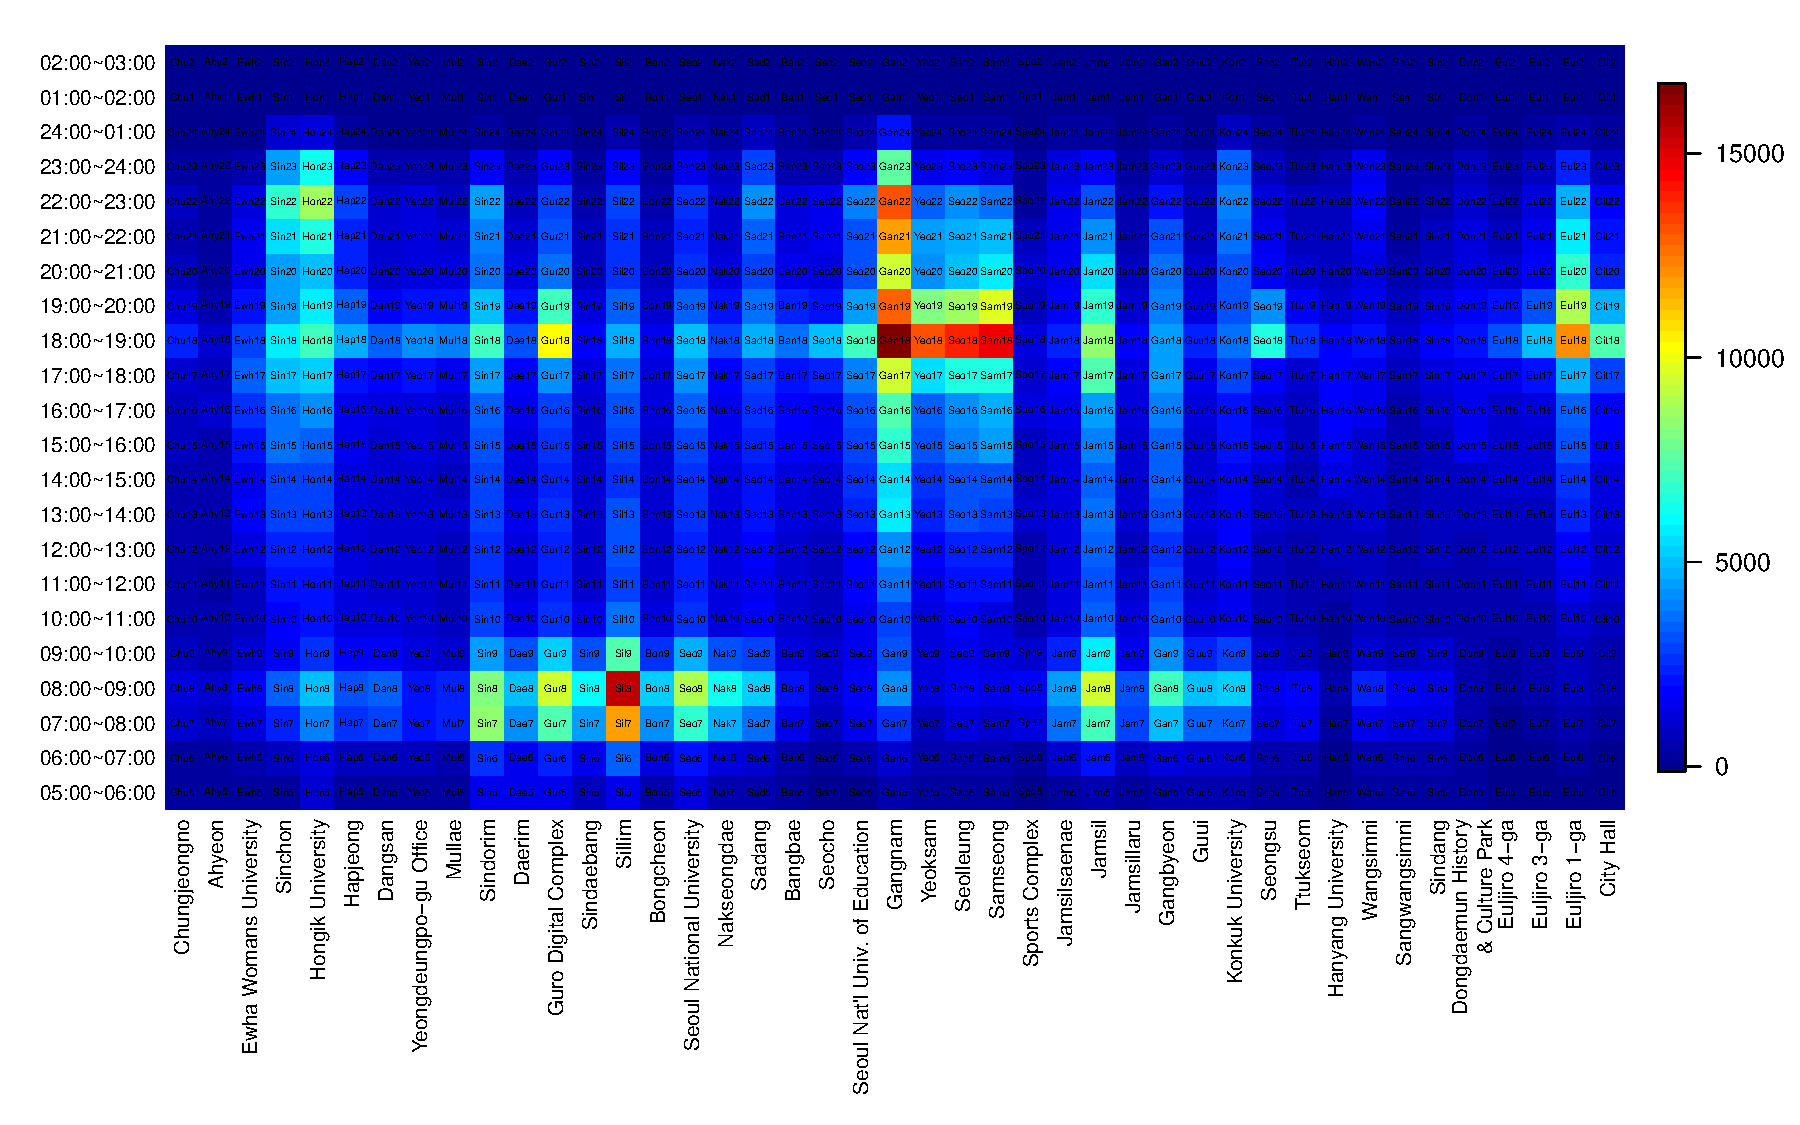
\includegraphics[width=1.05\textwidth]{Fig/In_data.pdf}
	\vspace{-13mm}
	\caption{Subway passenger data of Seoul Metro Line 2 in March 7, 2014.}
	\label{snow:subway_in_0}
\end{figure}	
%\end{sidewaysfigure}

So the exact data structure looks like Figure \ref{snow:datasrt}. Each point connected with temporally, and spatially. So this is a spatio-temporal data. If we fixed time then this is the circular data, and if we fixed the station then this data is time series. 

\begin{figure}
\centering
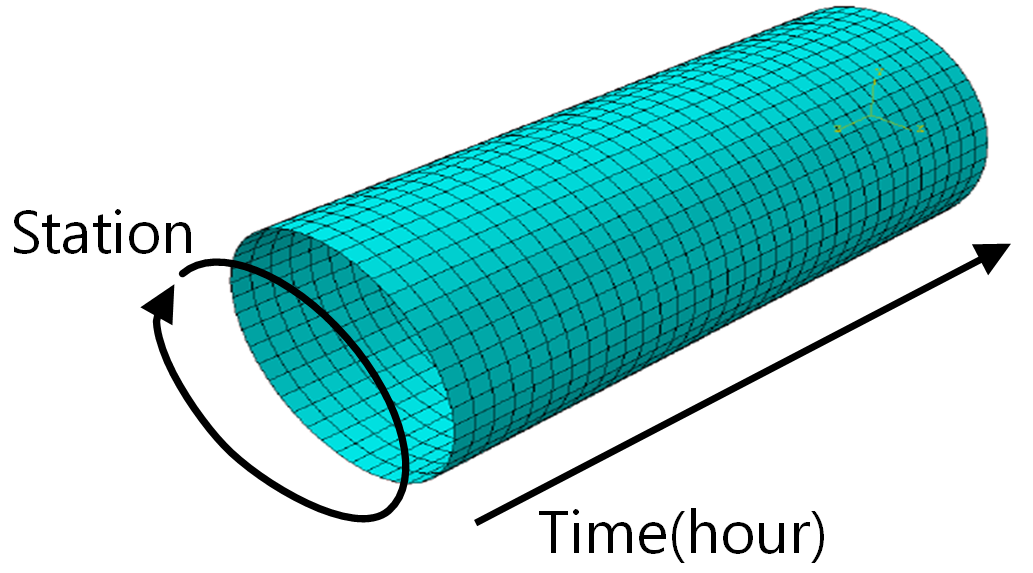
\includegraphics[width=1\textwidth]{Fig/data_str.png}
\vspace{-13mm}
\caption{Data structure of subway passenger data with Seoul metro line 2 in March 7, 2014.} 
\label{snow:datasrt}
\end{figure}

\noindent\textbf{\underline{Oneday analysis}}

Figures \ref{snow:subway_in_01} to \ref{snow:subway_in_5} show the importance plot of subway passenger data with ${\cal T}=10,100,200,300,400,500$. In local scale analysis, the most important cell is Gangnam station at 6 pm. It looks like a very reasonable result because Gangnam station is considered the hottest place in Seoul at that time. In addition to Gangnam station, some stations or group of stations are also considered to be important. In the morning of rush hour time, the residence area such as Sindorim, Guro Digital Complex, Sillim, Seoul National University and Jamsil stations are considered to be important. In the evening of rush hour time, the office area such as Guro Digital Complex, Gangnam, Yeoksam, Seolleung, Samsung and Euljiro 1-ga are considered to be important as well. 

When growing scale up to ${\cal T}=300$, the importance of Euljiro 1-ga station surpass the Gangnam station, and in the case of  growing scale more, the importance of Sillim station surpasses the Gangnam and Euljiro 1-ga stations. Why the importance of each cell changes over scale ? Look at the Figure \ref{snow:subway_in_0} again. We easily check that vertical array from Gangnam station at 18:00 to Gangnam station at 24:00 have high values, and we also check that horizontal array from Gangnam station at 18:00 to Samsung station at 18:00 have high values, too. Thus, we expect that the value of Gangnam station at 18:00 will be high since it is cross point of those two arrays. But, the situation is something different in Sillim station at 7:00--9:00. The values of these two cells cannot be expected by any linked data because these are extremely high than other linked cells. In summary, the value of Gangnam station at 18:00 can be expected by linked data, but those of Sillim station at 7:00--9:00 cannot be expected by linked data. So if we examine data with global scale, that means if we more widely consider the linked data, then the value of Gangnam station at 18:00 is more predictable than Sillim stations at 7:00-9:00. Thus the value of Gangnam station is less important than Sillim station.

\noindent\textbf{\underline{Type of area: commercial, residential, and office area.}}

\noindent\textbf{\underline{When is the peak time for each region?}}

\noindent\textbf{\underline{What is the most important day of the week in each region??}}

\subsubsection{Messenger data} 

\noindent\textbf{\underline{Data dercription.}}

\noindent\textbf{\underline{Who is influential?}}

\noindent\textbf{\underline{What is important Month?}}

\noindent\textbf{\underline{Change of relationship.}}

\noindent\textbf{\underline{Recommendation.}}



\section{Concluding Remarks}
Heavy-snow transform is a new multiscale visualization technique which is motivated by observing how snowfall accumulates. The concept of heavy-snow transform is shared with that of scale-space theory in computer vision. Heavy-snow transform is useful for evaluating some probabilistic structures of linked data whether a particular set of observations is similar to nearby other or not. We define the dissimilarity of the data and define the importance of the data based on it. We also introduced useful applications such as change-point detection and smoothing.

\iffalse
Another interesting key point is that the heavysnow transform have a \emph{multiscale} attribute. In (b), the case of least snow falling ($\tau=20$) relatively identifies the detailed features of underlying function, while the case of most snow falling ($\tau=160$) captures the global trends of it. In other words, the snowy grounds constructed by different $\tau$'s hold multiscale concept that can be interpreted as ``zoom-in" and ``zoom-out" of the signal. As one can see, the amount of snow accumulation is closely related to the resolution of data visibility, so $\tau$ can be considered as a multiscale parameter in scale-space analysis.

This multiscale attribute of heavysnow transform allows us to accept various points of view that define the dissimilarity between data. To better understand, consider the example in Figure 3. This example will be analyzed later in section xx, so we will omit details here. Groups A, B, and C, shown in the upper left of Figure 3, were generated from normal distributions with mean $0$, $1$, and $5$, respectively. Our question is:  
 Which group looks the least similar to the others? Although the question is simple, there may be several answers to this question. For example, the following answers are possible:
\begin{itemize}
\item \textbf{\it First point of view (average distance between clusters):} The C group is the most different from other groups. Because A's mean is 0 and B's mean is 1, so there is no big difference between them, but the mean of C is 5, which is much larger than the mean of A and B.
\item \textbf{\it Second point of view (rarity, outlier):} Group B is the most unusual group. Because observations belonging to group B are rarer than other groups. (The number of observations in group A and C is 400 and 50, respectively, but the number of observations in group B is XX)
\item \textbf{\it Third point of view (change point):} The points at the border of group A and group C are most unusual. This is because  sudden mean change occurs at this point.
\end{itemize}
Each point makes sense. The first perspective is suitable for clustering data according to specific criteria. The second point of veiw consider the scarcity of the data. Thus, it can be applied to outlier detection. (If there is only one point belonging to group B, this one point can be seen as outlier.) The third perspective can be used to detect change point. 

Figure 3 (b)-(d) show the dissimilarity of the given data. The proposed method can produce various viewpoints by controlling the multiscale parameter $\tau$,  and viewpoints depicted in Figure (b) to (d) are the results of our proposed visulization techneque described in section XX. As you can see, since heavysnow transform has the property of multiscale, it is possible to express various views of dissimilarity by only adjusting $\tau$.

\begin{figure}
\centering
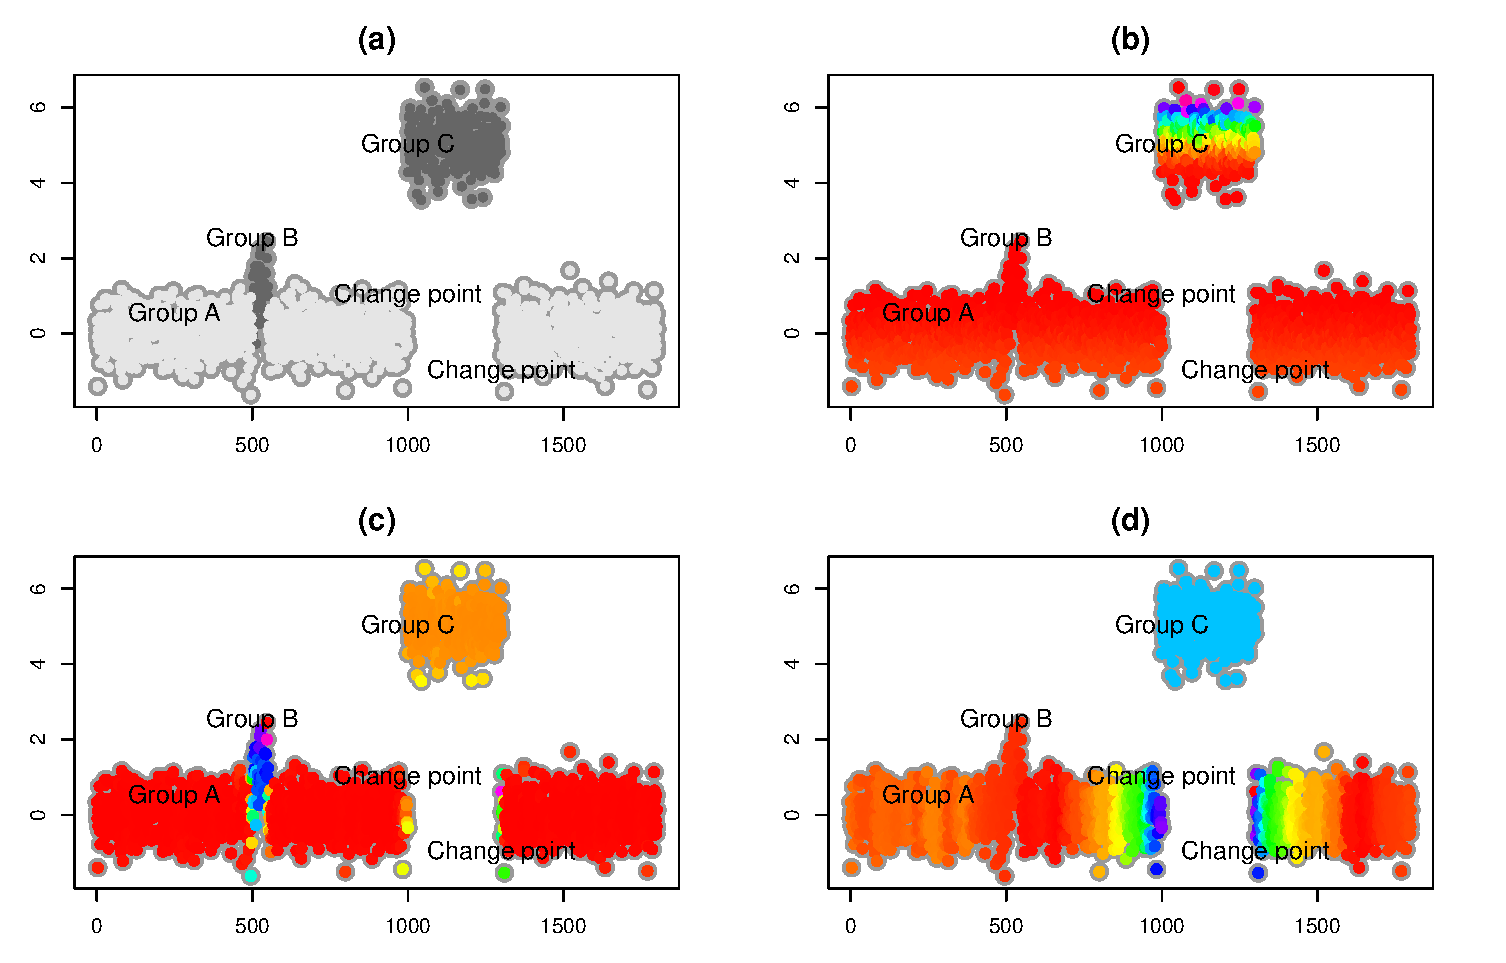
\includegraphics[width=1\textwidth]{Fig/Fig3.pdf}
\caption{(a) Observed data in Example XX. (b)-(d): Importance plot of (a) for $\tau=10, 200$, and $1200$, respectively. The points with no special differences compared to the other points are colored in red, and the special points distinguishing from other points are marked in purple.}
\end{figure}

이상검출은 비유사성의 개념과 밀접한 관련이 있다. Breunig(2000)은 두 자료간의 비유사성을 측정하고 이를 활용하여 자료의 이상성을 측정하는 새로운 기준인 local outlier factor를 제시하였다. 그 외에도 비유사성과 이상성을 함께 연구한 수많은 연구가 있다. 하지만 이러한 이상검출기법은 미리 정해진 규칙(자료의 무리로부터 떨어진 점을 이상점으로 간주)에 따라 이상값을 찾아내는 비지도학습형태의 기법이므로 미리 정해진 규칙이 이용자의 의도와 맞지 않는 경우 적절하게 이상값을 검출해 낼 수 없다. 본 연구에서 다루는 방법은 인덱스집합의 구조를 고려하는 정도에 따라 이상점을 판단하는 규칙을 변경할 수 있다는 장점이 있어 이용자의 의도와 맞는 이상점을 검출해낼 가능성이 높다. 또한 일반적인 산점자료에서 수행되는 이상검출과 달리 자료의 인덱스의 구조를 함께 고려하는 특징으로 인하여 변화점탐지를 마치 이상점탐지와 같은 기법으로 수행할 수 있다는 장점이 있다.  
* 그림2의 관점3에서 탐지되는 변화점은 기존의 이상점탐지와 동일한 기법으로 수행된 것임.

\noindent\textbf{(2) 차원축소와 클러스터링}

차원축소란 고차원의 자료가 가지는 본질적인 정보를 가능한 유지하면서 저차원의 자료로 변환하는 기법이다. 하지만 일반적인 차원축소는 원래자료가 가지고 있던 유사도를 손실하는 경우가 있어 자료간의 유사성을 보존하면서 차원축소를 하려는 연구가 활발히 진행되었다. He, X (2004)는 입력표본간의 유사도를 이용한 새로운 차원 축소기법을 제안하였으며 Belkin (2003)는 유사도행렬을 활용한 새로운 차원축소기법을 제안하여 swiss-roll 형태의 매니폴드를 가지는 자료를 2차원 공간으로 효과적으로 맵핑하는 기법을 소개하였다. Ng. A.Y. (2002)는 자료간 유사도를 유지하는 차원축소를 수행하고 통상적인 K-평균 클러스터링을 수행하는 알고리즘을 소개하였다. 이러한 기법들의 핵심은 유사도행렬을 활용하여 차원축소기법에서 자료의 매니폴드를 효과적으로 유지하다는 것에 있다. 하지만 기존의 유사도행렬은 인덱스집합의 구조에 따라 달라지는 비유사성을 포착하기 불가능하다는 단점이 있으며 이는 자료의 매니폴드를 구체화하는 표현력을 억제한다. 반면 제안된 방법을 활용하면 다양한 매니폴드에서 정의된 자료에 대한 거리를 이용자의 의도에 맞게 재정의할 수 있어 다른 공간으로 맵핑시킬 때 이를 효과적으로 표현가능하다는 장점이 있다.

\noindent\textbf{(3) 멀티스케일 디콤포지션} 

From the above example, we describe a brief idea of the proposed transformation and present its preliminary definition that represents data over various scales by $\tau$ and performs some useful data analysis. The main advantages of the proposed transformation is two-fold: (a)  A particular multiscale approach (transformation) is typically designed for a specific group (class) of data such as one-dimensional data (sequence, line) or two-dimensional data (two-array object, plane). In some sense, the scope of data structure that can be handled by a multiscale method is limited. On the other hand, the proposed transformation extends the scope to `linked data' that cover a wide class of data, which will be defined later. Roughly speaking, the heavy-snow transform can be applicable to any data structure that snow can be accumulated. (b) We present new two measures based on the proposed transformation, termed dissimilarity and importance, which utilize the inherent characteristics of the transformation; hence, these are useful for identifying and analyzing various data, and  further are applicable to some application such as smoothing or detection problem.   

In literature, there exist numerous multiscale methods that may share a multiscale concept of the proposed method. SiZer by Chaudhuri and Marron (1999) is a visualization technique that displays smoothed data as a function of location and bandwidth over a range of bandwidths, which is motivated by the `scale-space' theory in computer vision (Lindeberg, 1994). Several attempts for variants of SiZer have been developed (Hanning and Lee, 2006; Hanning et al., 2013; Park et al., 2009, Park et al., 2010). Moreover, many scale-space methods have been studied. For an extensive review of statistical scale-space methods, see Holmstr\"oma (2010) and Holmstr\"oma and Pasanena (2017). As another scale-space method, Fryzlewicz and Oh (2011) proposed thick-pen transformation which plots time series data over a range of thickness values of pen. As other direction of multiscale methods, wavelet transformation has been extensively studied for representation of inhomogeneous one- or two-dimensional data. For details of wavelets in statistics, see  Vidakovic (1999) and Nason (2010). 

The remaining of this paper is organized as follows. Section 4.2 defines heavy-snow transformation and proposes some statistics based on heavy-snow transformation, dissimilarity and importance of data for statistical data analysis. In Section 4.3, numerical experiments including real data analysis are presented. As for a challengeable aspect, Seoul Metro passenger data that are a kind of cylinder data structure are used. Finally, concluding remarks are given in Section 4.4 where a possible use for smoothing is briefly discussed as a future research topic. 
\fi 


\section*{Appendix}
\subsubsection*{Figures}

%\begin{sidewaysfigure}
\begin{figure}
	\centering
	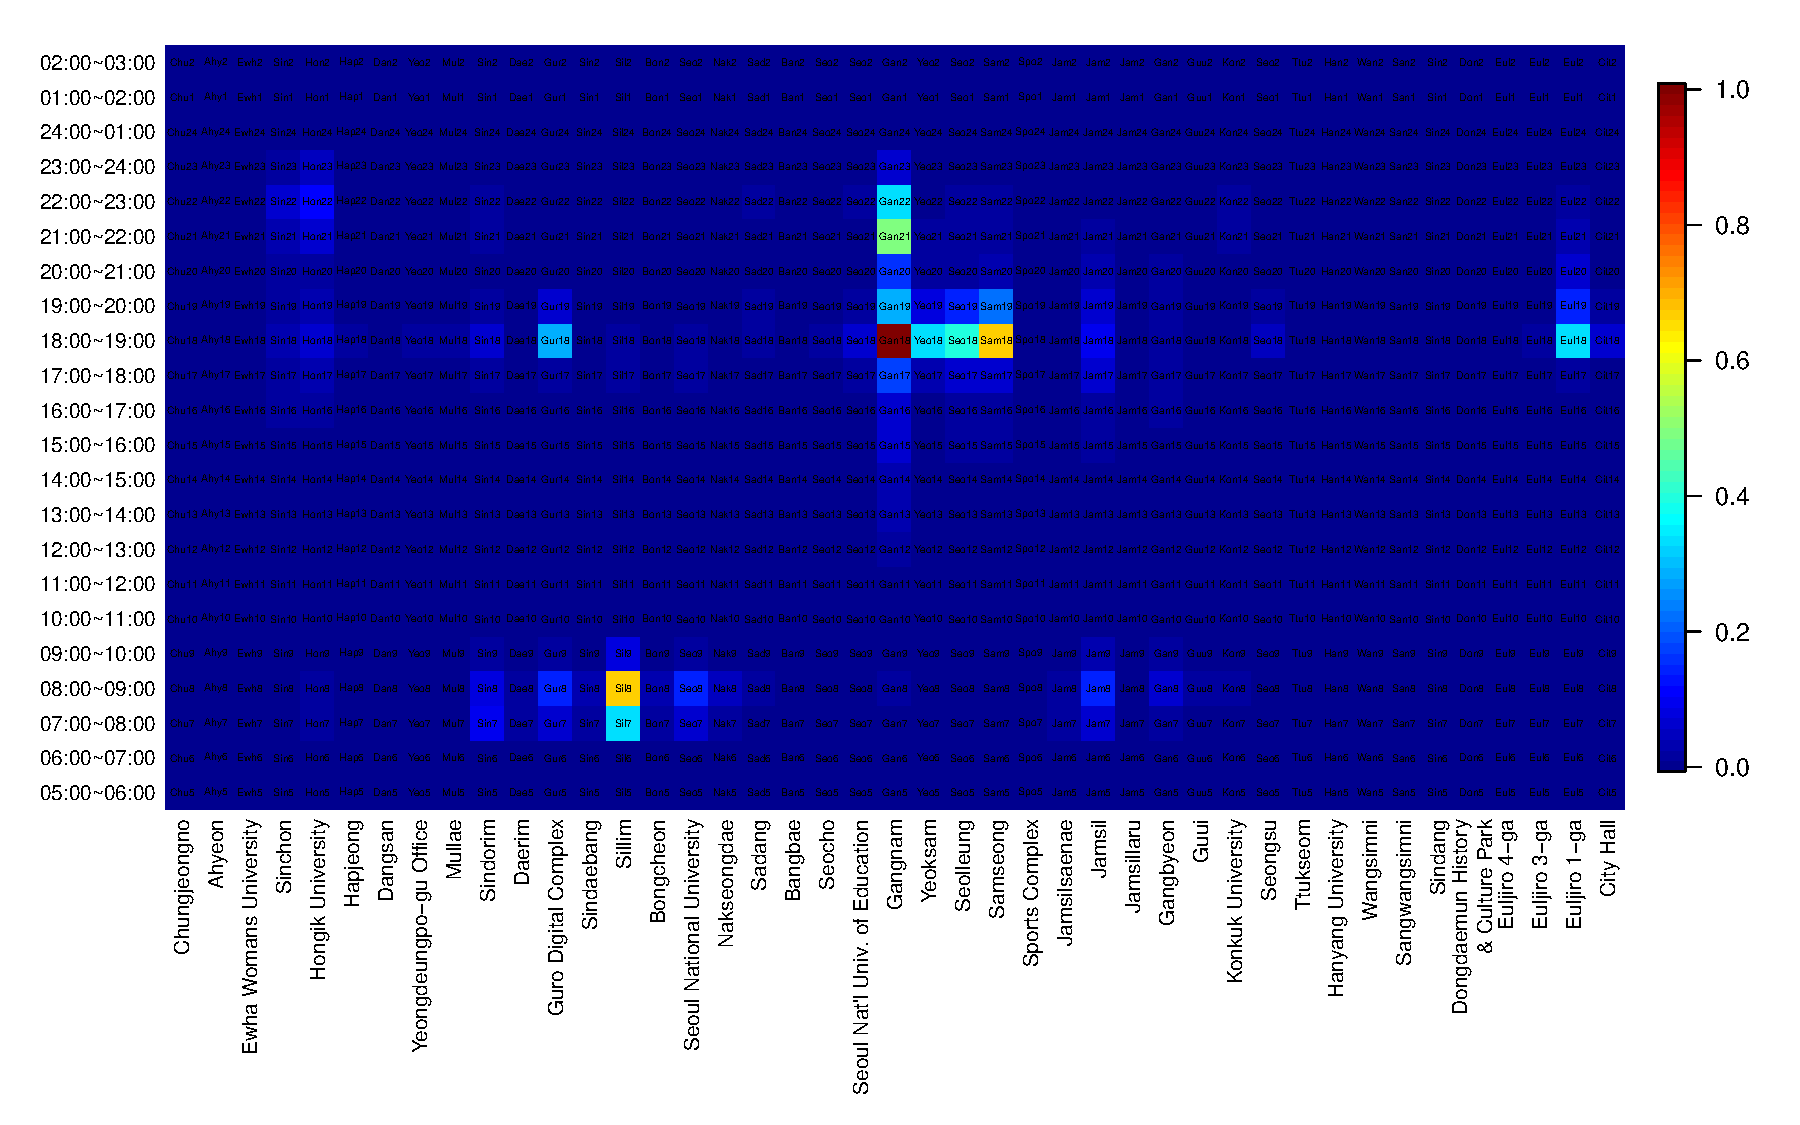
\includegraphics[width=1.05\textwidth]{Fig/In_scale_1.pdf}
	\vspace{-13mm}
	\caption{Importance plot of subway passenger data with ${\cal T}=10$.}
	\label{snow:subway_in_01}
\end{figure}
%\end{sidewaysfigure}

%\begin{sidewaysfigure}
\begin{figure}
	\centering
	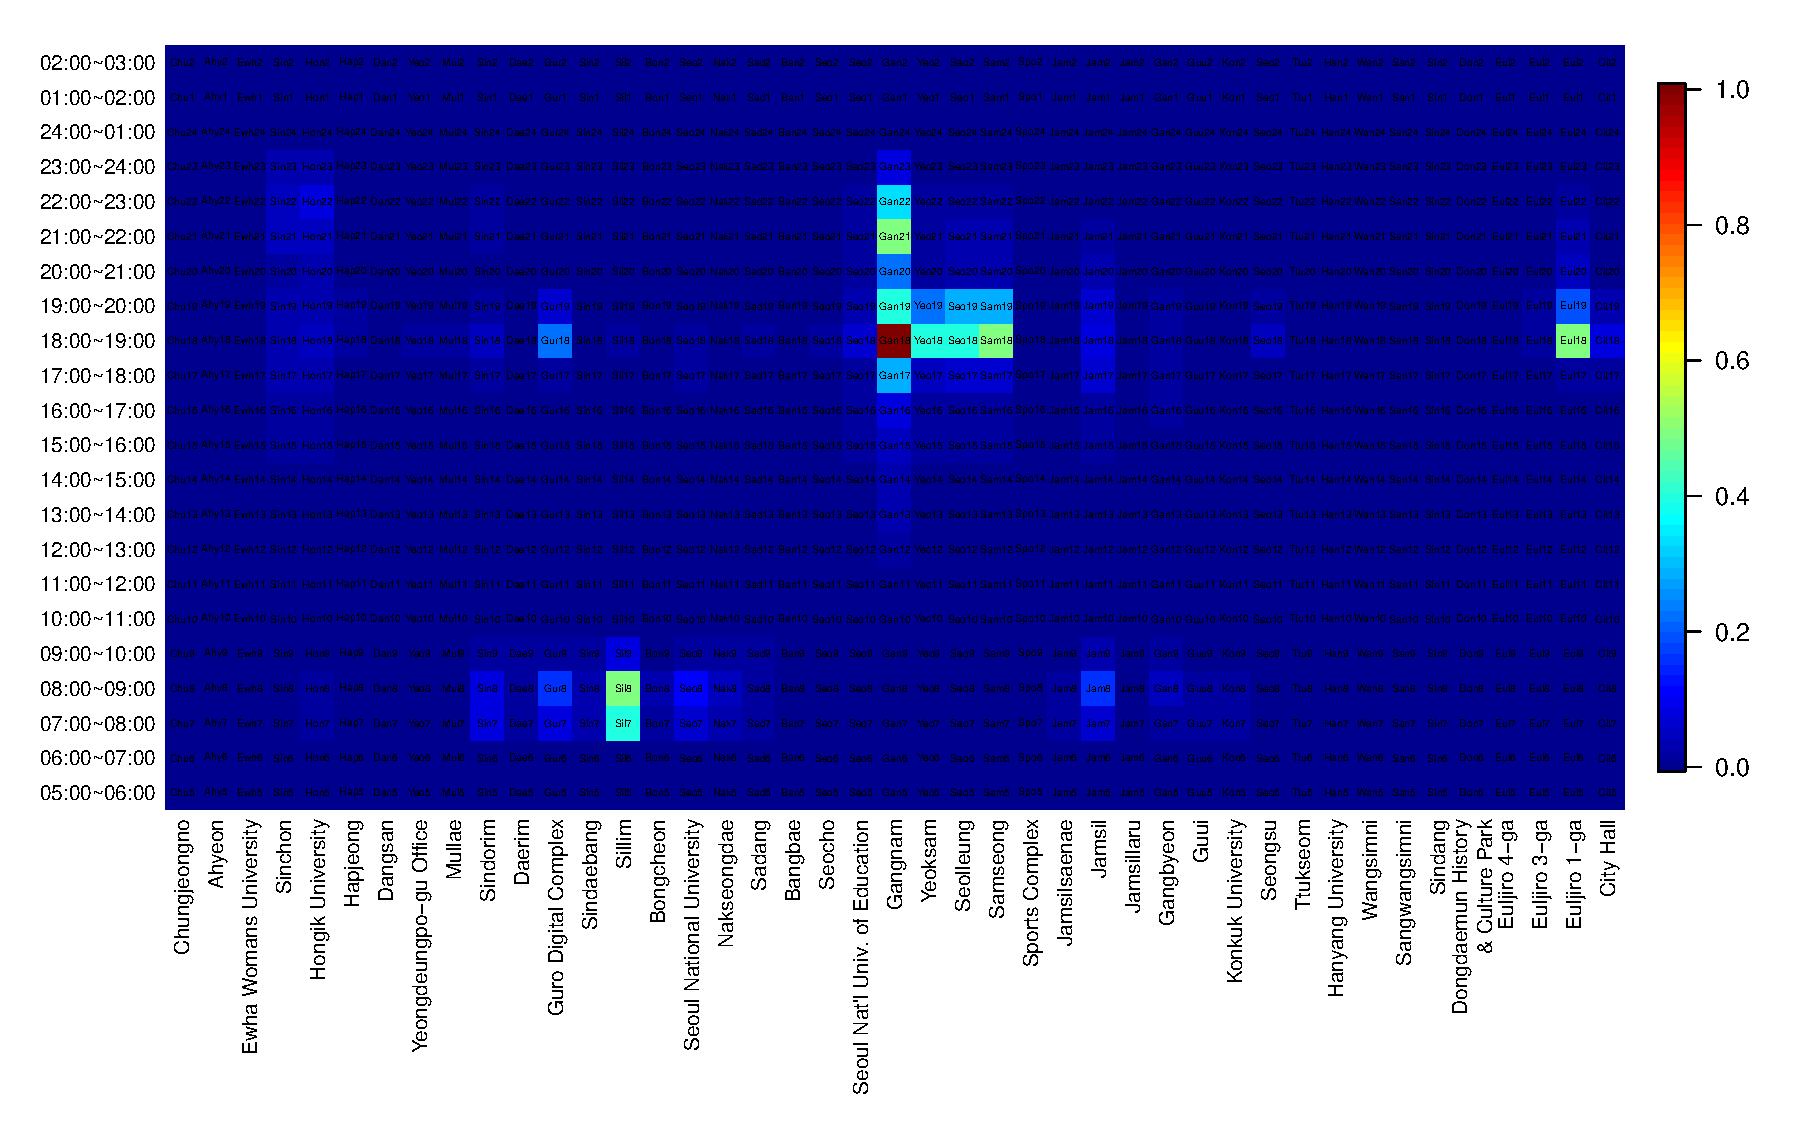
\includegraphics[width=1.05\textwidth]{Fig/In_scale_2.pdf}
	\vspace{-13mm}
	\caption{Importance plot of subway passenger data with ${\cal T}=100$.}
	\label{snow:subway_in_1}
\end{figure}
%\end{sidewaysfigure}

%\begin{sidewaysfigure}
\begin{figure}
	\centering
	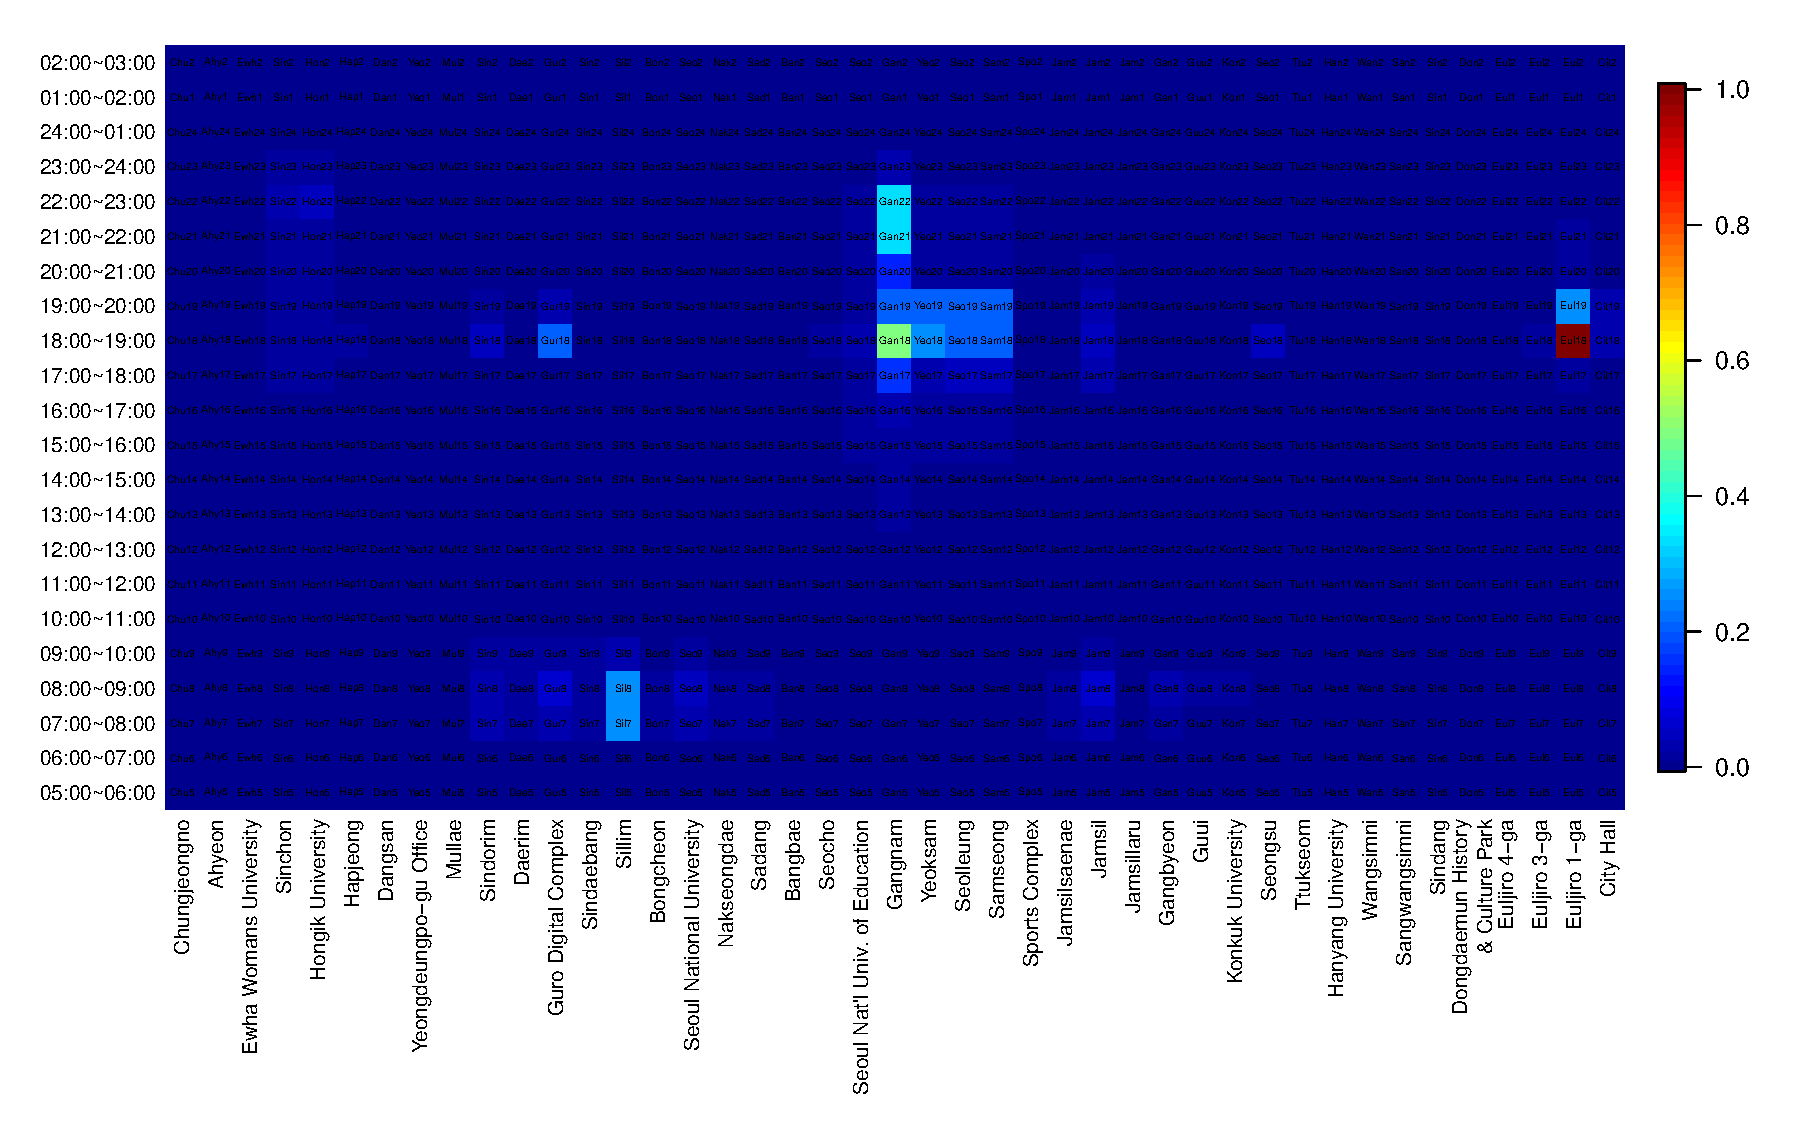
\includegraphics[width=1.05\textwidth]{Fig/In_scale_3.pdf}
	\vspace{-13mm}
	\caption{Importance plot of subway passenger data with ${\cal T}=200$.}
	\label{snow:subway_in_2}
\end{figure}
%\end{sidewaysfigure}

%\begin{sidewaysfigure}
\begin{figure}
	\centering
	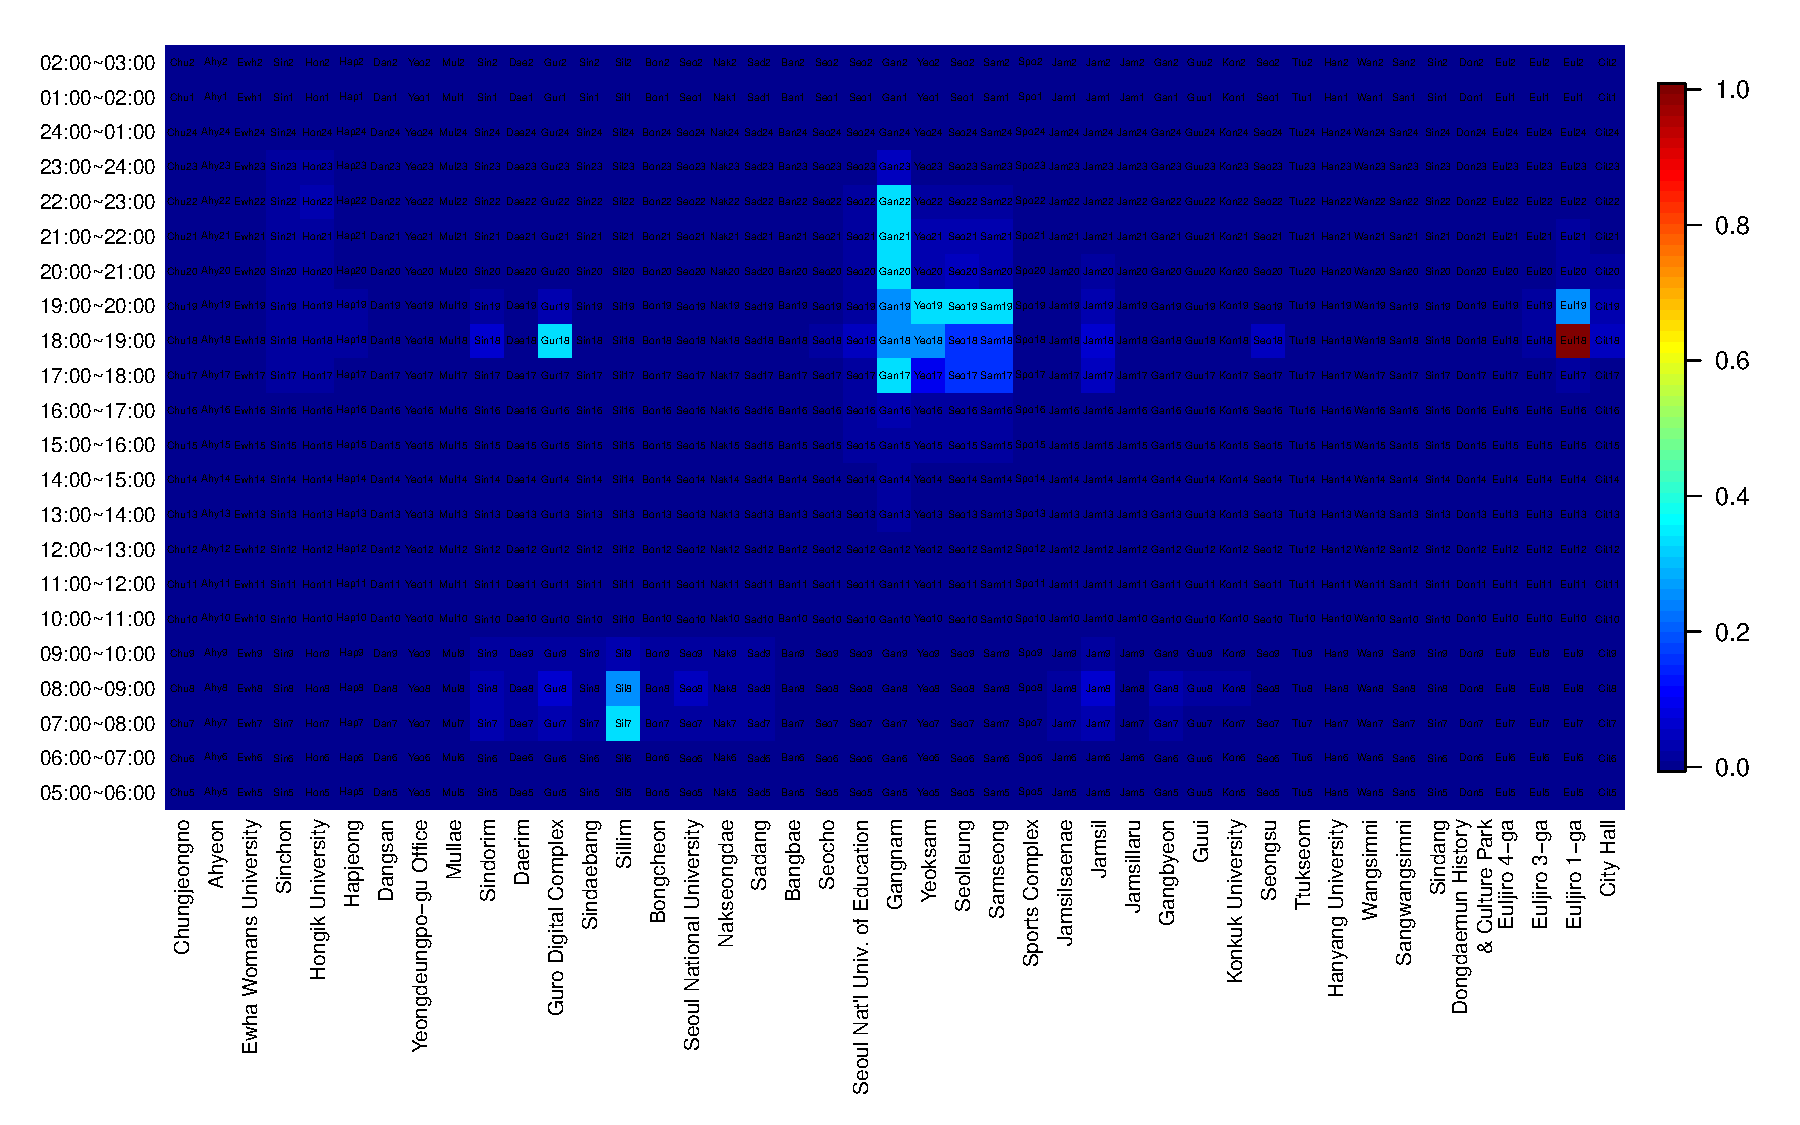
\includegraphics[width=1.05\textwidth]{Fig/In_scale_4.pdf}
	\vspace{-13mm}
	\caption{Importance plot of subway passenger data with ${\cal T}=300$.}
	\label{snow:subway_in_3}
\end{figure}
%\end{sidewaysfigure}

%\begin{sidewaysfigure}
\begin{figure}
	\centering
	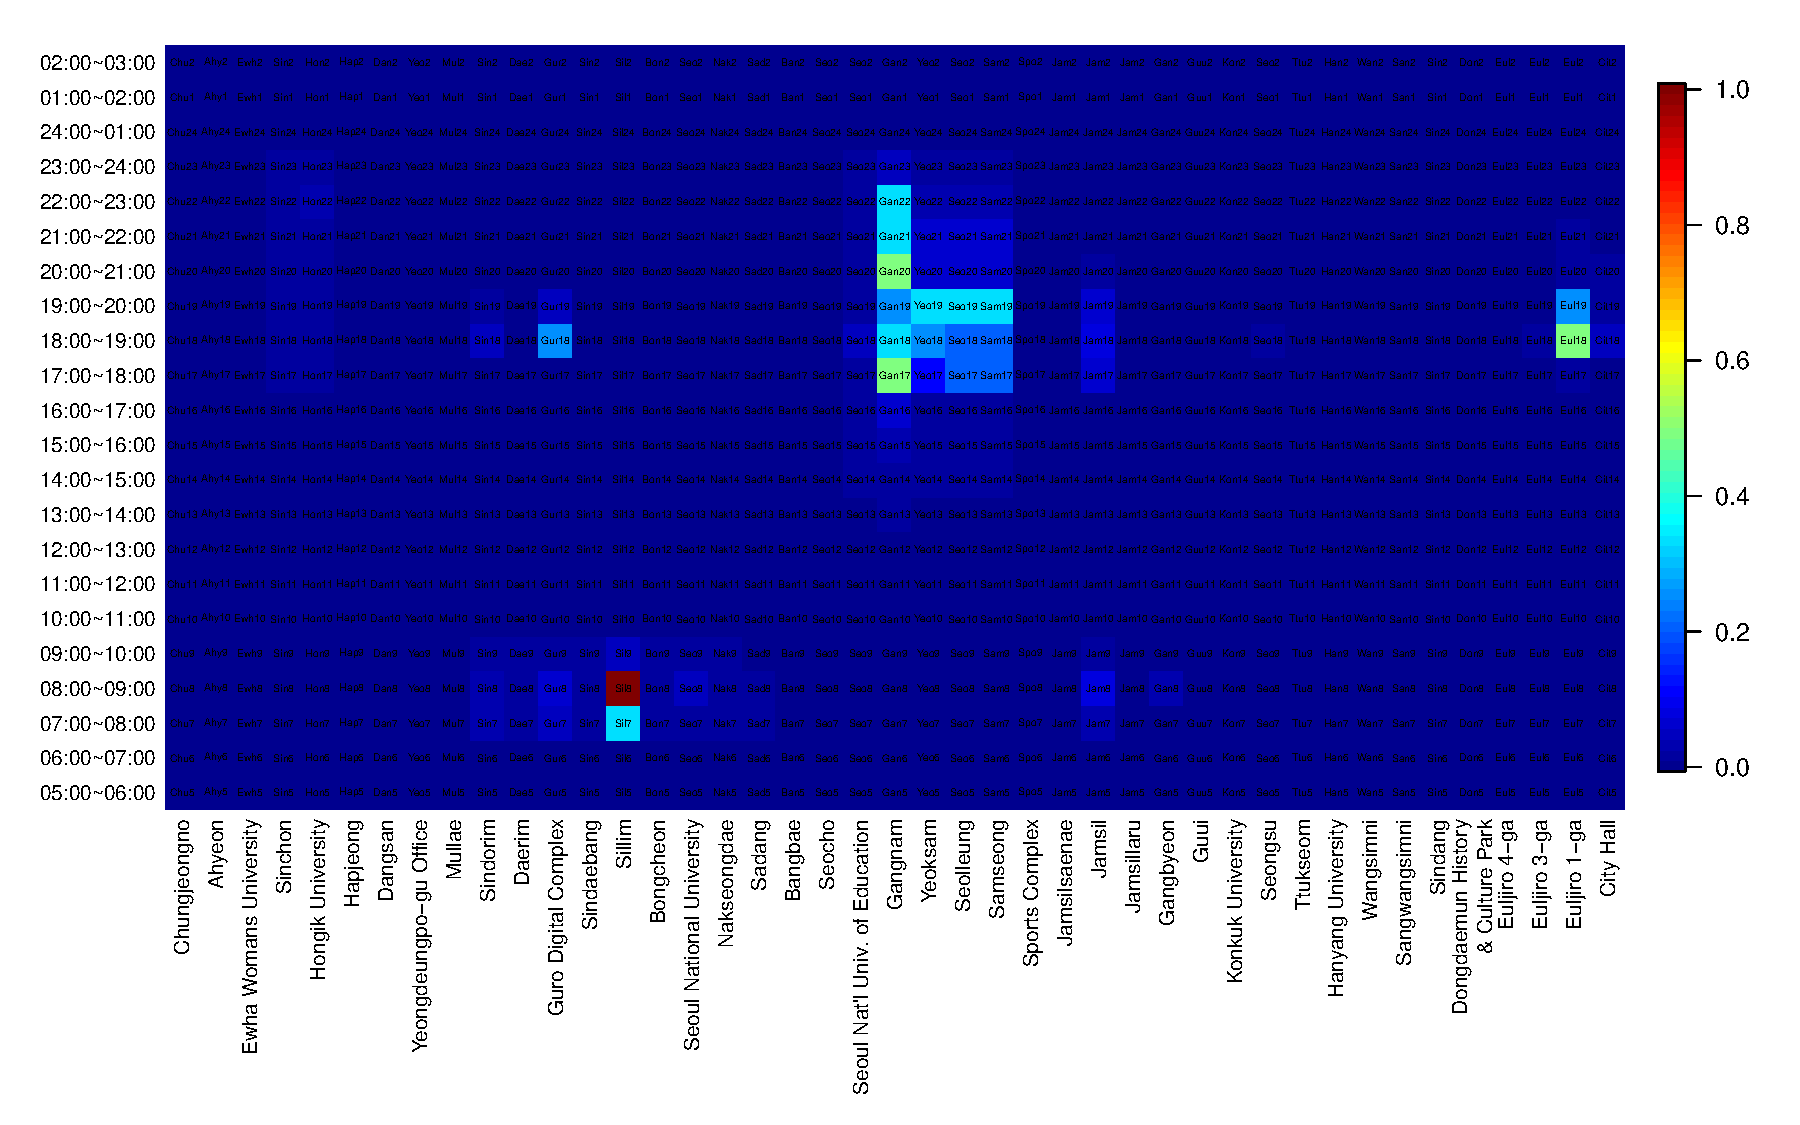
\includegraphics[width=1.05\textwidth]{Fig/In_scale_5.pdf}
	\vspace{-13mm}
	\caption{Importance plot of subway passenger data with ${\cal T}=400$.}
	\label{snow:subway_in_4}
\end{figure}	
%\end{sidewaysfigure}

%\begin{sidewaysfigure}
\begin{figure}
	\centering
	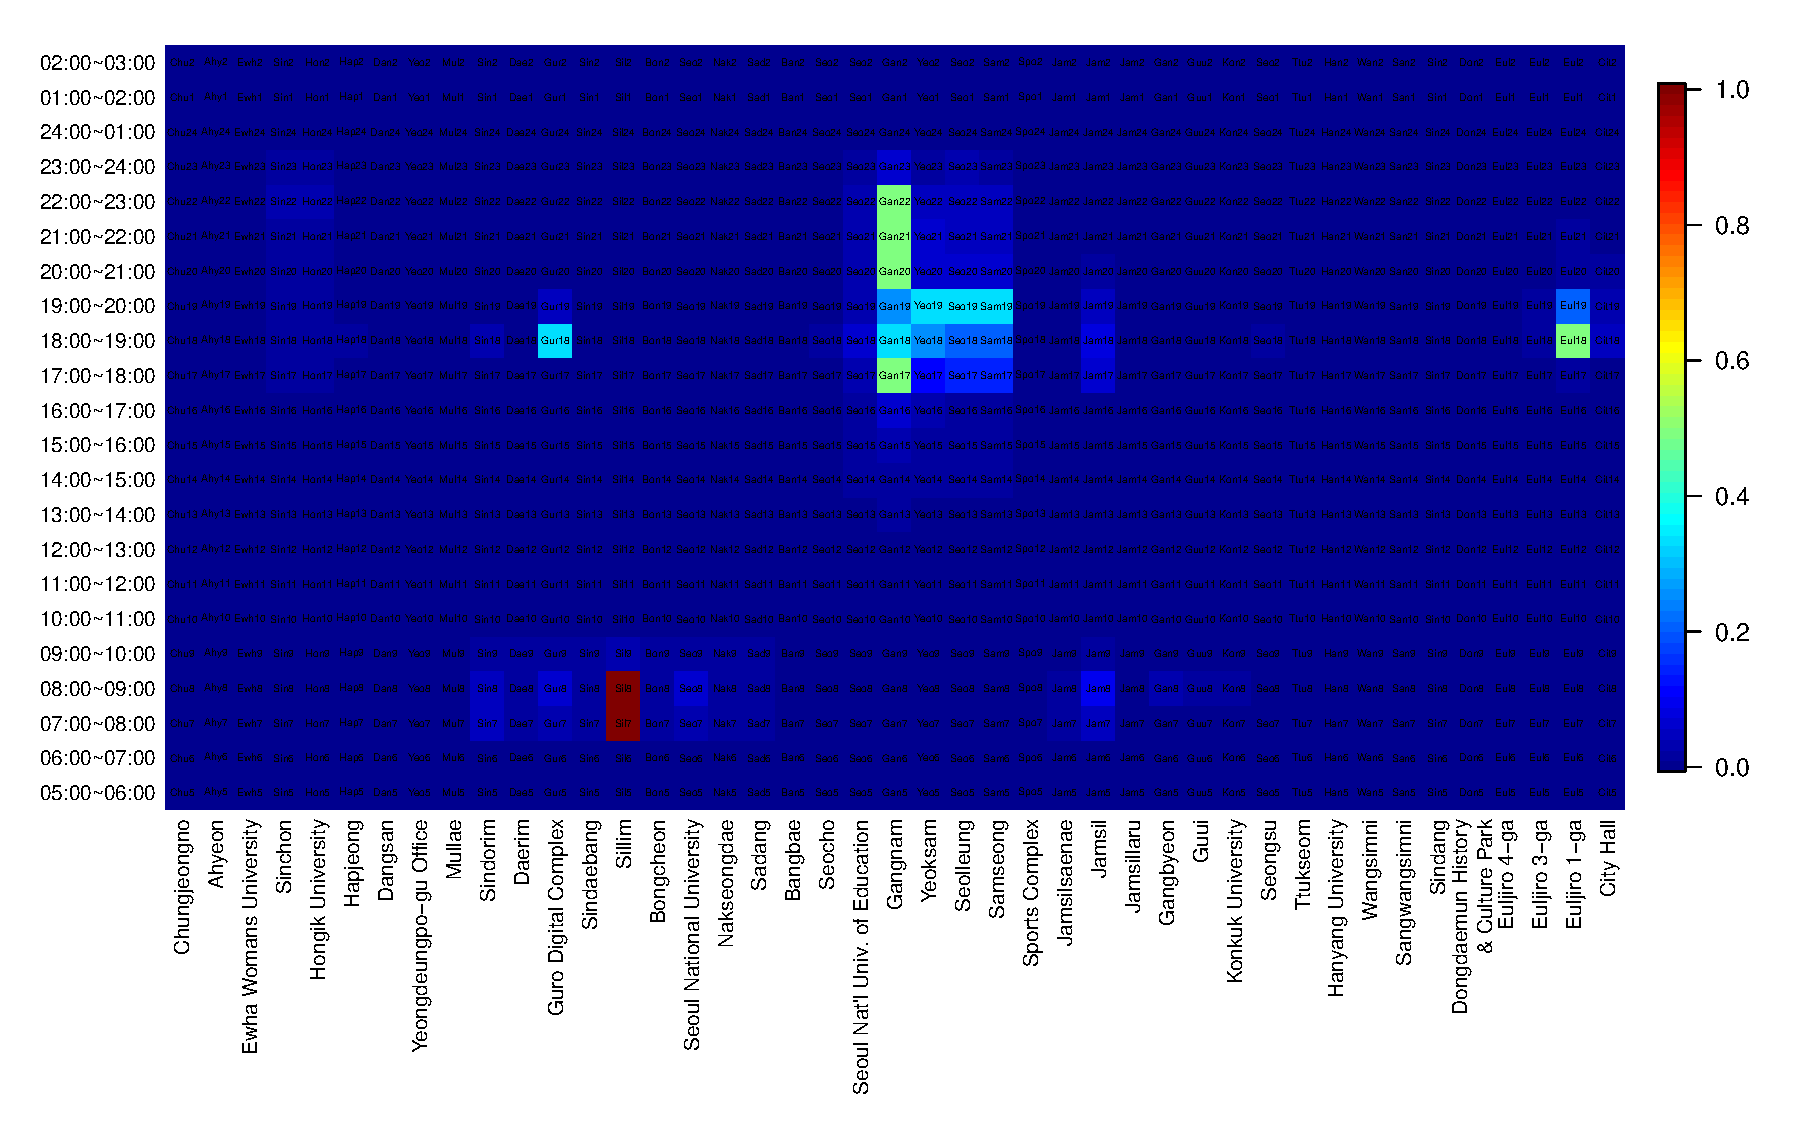
\includegraphics[width=1.05\textwidth]{Fig/In_scale_6.pdf}
	\vspace{-13mm}
	\caption{Importance plot of subway passenger data with ${\cal T}=500$.}
	\label{snow:subway_in_5}
\end{figure}	
%\end{sidewaysfigure}	


\section*{Appendix}
\subsubsection*{Smoothing}

- 여기에서는 헴펠교재 P.316 의 내용을 참고하였다. 선형모델에서 모수 $\boldsymbol{\beta}$의 추정량 $\boldsymbol{\beta}_ n$ 을 구하는 것은 아래를 푸는 것이고 
\begin{align}
\min_{\boldsymbol{\beta}_ n}\sum_{i=1}^{n}\rho(y_i-{\bf x}_ i \boldsymbol{\beta}_ n)
\end{align}
이것은 다시 아래의 방정식의 해를 푸는것과 같다. 
\begin{align}
\sum_{i=1}^{n}{\bf x}_ i^T\psi\big(y_i-{\bf x}_ i \boldsymbol{\beta}_ n\big)=0 
\end{align}
이런 추정량 $\boldsymbol{\beta}_ n$을 $M$-estimator라고 한다. 일반적인 회귀분석 모형에서는 $\psi(y)=y$ 가 되어 위의 식은 
\begin{align}
\sum_{i=1}^{n}{\bf x}_ i^T\big(y_i-{\bf x}_ i \boldsymbol{\beta}_ n\big)=\sum_{i=1}^{n}{\bf x}_ i^T y_i-\sum_{i=1}^{n}{\bf x}_ i^T {\bf x}_ i \boldsymbol{\beta}_ n= {\bf X}'{\bf y}-{\bf X}'{\bf X}\boldsymbol{\beta}_ n=0 
\end{align}
와 같이 정리된다. 따라서 $\boldsymbol{\beta}_ n = ({\bf X}'{\bf X})^{-1}{\bf X}'{\bf y}$ 와 같이 정리된다.

- 반면 generalized $M$-estimator 는 아래를 최소화하는 해이다. 
\begin{align}
\sum_{i=1}^{n}{\bf x}_ i \phi\big({\bf x}_ i , y_i-{\bf x}_ i \boldsymbol{\beta}_ n\big) =0 
\end{align}
여기에서 $\psi$는 $1\times p$ row-vector를 실수로 보내는 맵핑이다. 즉 $\psi:\mathbb{R}\times \mathbb{R}^p \to \mathbb{R}$ 이다. 만약에 
\begin{align}
\phi({\bf x},u)=\psi(u)
\end{align}
를 만족하면 이 경우 generalized $M$-estimator 는 classical $M$-estimator 와 같다. 

- 이때 $\sum_{i=1}^{n}{\bf x}_ i \phi\big({\bf x}_ i , y_i-{\bf x}_ i \boldsymbol{\beta}_ n\big) =0$ 은 아래와 같이 쓸 수 있다. 
\begin{align}
\int {\bf x} \phi\big({\bf x} , y-{\bf x} \boldsymbol{\beta}\big) dF_n=0 
\end{align}

- WLS의 경우 
\begin{align}
\boldsymbol{\beta}_ n = \big({\bf X}'{\bf W}^2{\bf X}\big)^{-1}{\bf X}'{\bf W}{\bf y}
\end{align}
와 같이 된다. 이런 경우는 $\psi(y;{\bf w}_ i {\bf X})= \pi({\bf w}_ i {\bf X}) $ 와 같이 선택되었다고 볼 수 있다. 

\subsubsection*{Maronna and Yohai (1981)}

- 일반적인 셋팅은 아래와 같다. (1.1) 
\begin{align}
y_i={\bf x}_ i \boldsymbol{\beta}  +\epsilon_i 
\end{align}
여기에서 $\epsilon_i$ 의 분산은 편의상 $1$ 로 가정한다. 

- 아래를 만족하는 $\boldsymbol{\beta}$ 를 구한다. (1.2) 
\begin{align}
\sum_{i=1}^{n}{\bf x}_ i \phi\big({\bf x}_ i , y_i-{\bf x}_ i \boldsymbol{\beta}_ n\big) =0 
\end{align}
이런 추정량 $\boldsymbol{\beta}_ n$을 $M$-estimator라고 한다. 여기에서 $\psi$는 $p\times 1$ row-vector를 실수로 보내는 맵핑이다. 

- 우리는 $y_i$ 대신 $f(v_i)$ 를 대입하고 ${\bf x}_ i$ 대신 $f(v_j),~ j\in\\{1,2,\dots,i-1,i+1,\dots,n\\}$ 를 대입한 셋팅을 생각하면 된다. 

- 참고문헌: Maronna and Yohai (1981), Damien Garcia (2010) 

- 적용자료: 지진자료 혹은 기상자료의 smoothing 을 수행하면 의미가 있어보인다. (시공간이 동시에 변화하는 자료들) 

- $\tau$ 의 선택??

\subsubsection*{Clustering}

- Spectral clustering 혹은 TDA식 클러스터링을 활용하거나 cut을 사용할 수 있다. 자료는 고민중.. 

- HST에 의한 라플라시안은 아래와 같이 정의할 수 있다. 
\begin{align}
{\bf L}_ {ij}^{(\tau)}=
\begin{cases} 
-w_{ij} & i\neq j \\\\ \\
\sum_k w_{ik} & i=j. 
\end{cases} 
\end{align} 
이때 
\begin{align}
w_{ij}=\begin{cases}
\exp \Big(-\frac{d_1^2(v_i,v_j)}{2b^2}\Big) & (i,j) \in E \\\\ \\
0 & o.w.
\end{cases}
\end{align}
이다. 여기에서 $b$는 bandwidth 를 의미한다. 눈이 올수록 점점 값이 커지니까 $b$를 $\tau$에 비례하여 증가시켜야 할것 같다. 

- 이제 $f(v_1),\dots,f(v_2)$ 에 대응하는 ***graph Laplacian quadratic form*** 은 아래와 같다. 
\begin{align}
s_2(f;\tau):=\sum_{(i,j)\in E} w_{ij} \big(f(v_i)-f(v_j)\big)^2={\bf f}^T {\bf L}^{(\tau)}{\bf f}
\end{align}
여기에서 ${\bf f}=(f(v_1),\dots,f(v_n))'$ 이다. 

- 만약에 $f(v_i)$가 랜덤이면 $W_{ij}$도 랜덤이 된다. 그리고 $S_2(f;\tau)$도 랜덤이 된다. 그리고 $f$ 와 $W$ 모두 ${\boldsymbol h}$ 가 정의되는 확률공간$(\Omega,{\cal F},P)$ 에서 정의할 수 있다. 참고로 ${\boldsymbol h}$ 에서 $f$, $W$, $S_2(f;\tau)$를 만드는 함수가 각각 연속함수가 되어 각각을 정의하는데 무리가 없다. 

\subsubsection*{Spectral Decomposition}
asdf




\begin{thebibliography}{}

%\bibitem{Aldroubi1992} Aldroubi, A., Unser, M., \& Eden, M. (1992). Cardinal spline filters: Stability and convergence to the ideal sinc interpolator. {\it Signal processing}, {\bf 28}, 127-138.

%\bibitem{Arino2004} Arino, M. A., Morettin, P. A., \& Vidakovic, B. (2004). Wavelet scalograms and their applications in economic time series. {\it Brazilian Journal of Probability and Statistics}, 37-51.

%\bibitem{Bertsekas1976} Bertsekas, D. P. (1976). Multiplier methods: A survey. {\it Automatica}, {\bf 12}, 133--145.
\bibitem{Klein}Klein, D. J., and Randić, M. (1993). Resistance distance. Journal of mathematical chemistry, 12(1), 81-95.

\bibitem{Shuman} Shuman, D. I., Narang, S. K., Frossard, P., Ortega, A., and Vandergheynst, P. (2012). The emerging field of signal processing on graphs: Extending high-dimensional data analysis to networks and other irregular domains. arXiv preprint arXiv:1211.0053.

\bibitem{Breunig} Breunig, M. M., Kriegel, H. P., Ng, R. T., and Sander, J. (2000, May). LOF: identifying density-based local outliers. In ACM sigmod record (Vol. 29, No. 2, pp. 93-104). ACM.
\bibitem{He} He, X., and Niyogi, P. (2004). Locality preserving projections. In Advances in neural information processing systems (pp. 153-160).

\bibitem{Belkin} Belkin, M., and Niyogi, P. (2003). Laplacian eigenmaps for dimensionality reduction and data representation. Neural computation, 15(6), 1373-1396.

\bibitem{Ng} Ng, A. Y., Jordan, M. I., and Weiss, Y. (2002). On spectral clustering: Analysis and an algorithm. In Advances in neural information processing systems (pp. 849-856).

\bibitem{Tsang} Tsang, I. W., and Kwok, J. T. (2007). Large-scale sparsified manifold regularization. In Advances in Neural Information Processing Systems (pp. 1401-1408).


\bibitem{Lafon} Lafon, S., and Lee, A. B. (2006). Diffusion maps and coarse-graining: A unified framework for dimensionality reduction, graph partitioning, and data set parameterization. IEEE transactions on pattern analysis and machine intelligence, 28(9), 1393-1403.

\bibitem{Leskovec} Leskovec, J., Lang, K. J., Dasgupta, A., and Mahoney, M. W. (2009). Community structure in large networks: Natural cluster sizes and the absence of large well-defined clusters. Internet Mathematics, 6(1), 29-123.

\end{thebibliography}
\end{document}